% =============================================================================
% Declined, displaced, or just harder to catch?
% Manuscript prepared for Fish and Fisheries (Original Article); thesis chapter.
%
% This file is the TEMPLATE. Lines of the form %%TAB:<name>%% are replaced by
% the LaTeX table bodies in results/tables/tex/<name>.tex when
%     Rscript scripts/assemble_manuscript.R
% writes manuscript/sim-rec_FishFisheries.tex, the file to compile.
% Figures are read from ../figures/ (repository) or figures/ (stand-alone).
% =============================================================================
\documentclass[11pt,a4paper]{article}
\usepackage[T1]{fontenc}
\usepackage{lmodern}
\usepackage[margin=25mm]{geometry}
\usepackage{amsmath,amssymb}
\usepackage{graphicx}
\graphicspath{{figures/}{../figures/}}
\usepackage{booktabs,array}
\usepackage[round]{natbib}
\usepackage{tikz}
\usetikzlibrary{positioning,arrows.meta}
\usepackage{setspace}
\onehalfspacing
\usepackage{lineno}            % line numbers for review; remove \linenumbers below for the thesis
\usepackage{caption}
\captionsetup{font=small,labelfont=bf,labelsep=period,justification=raggedright,singlelinecheck=false}
\usepackage[hidelinks]{hyperref}
\usepackage{xurl}
\setlength{\emergencystretch}{2em}
\newcommand{\vt}[1]{\text{#1}}
\setcounter{secnumdepth}{3}

\title{Declined, displaced, or just harder to catch? A simulation framework for attributing marine heatwave impacts on fished populations from catch per unit effort}
% Author list, affiliations and ORCIDs to be completed by the authors.
\author{}
\date{}

\begin{document}
\maketitle
\linenumbers

\noindent\textbf{Running title:} Attributing heatwave signals in catch rates

\begin{abstract}
\noindent Marine heatwaves are increasingly linked to declines in fished populations, and catch per unit effort (CPUE) is the signal most often used to detect them. A fall in CPUE during a heatwave can mean three things: fewer fish, fish that have moved away from the fishing grounds, or fish that are still present but harder to catch. Each calls for a different management response, but a real catch rate is never observed split into these parts. We used simulation, where it is known. Fishery data alone cannot separate a change in total abundance from a spatially uniform change in catchability, however much data are collected, whereas a catchability change confined to the warm edge is detectable. In a simulated fishery where abundance, distribution and catchability respond to the species' thermal niche and the fleet targets expected catches, we crossed abundance decline, redistribution, catchability loss and fleet contraction in a factorial design (400 replicates per scenario). No fishery index was robust to uniform catchability loss. When catchability did not change, a spatial delta model removed most of the redistribution bias, a partial fishery-only remedy that catchability loss lacks. A fishery-independent survey was unbiased for abundance inside the sampled area but could not see fish that left it, and only its centre of gravity separated real movement from a warm-edge catchability artefact. Sampling frequency mattered more than station count: monthly surveys of 7 to 14 stations outperformed every fishery index. Attributing heatwave impacts from catch rates is therefore a monitoring design problem.
\end{abstract}

\noindent\textbf{Keywords:} catch per unit effort; catchability; identifiability; marine heatwave; operating model; survey design

% =============================================================================
\section{Introduction}

Marine heatwaves, discrete periods of anomalously warm water, have become a defining feature of ocean change \citep{hobday2016}. They have lengthened and intensified over the past century \citep{oliver2018}, are projected to become more frequent and severe under continued warming \citep{frolicher2018,afrifa2026}, and now rank among the most acute threats to marine biodiversity and the services it supports \citep{smale2019}. Their biological consequences range from mass mortality and habitat loss to community reorganisation and shifts in species distributions \citep{wernberg2013,wernberg2016,babcock2019,cheung2020}. The 2010--11 Western Australian heatwave shows what is at stake for fisheries: it was followed by major recruitment failures in scallop, prawn and blue swimmer crab stocks, managers responded with effort reductions and spatial or temporal closures, and the assessment of that response called for early detection of abundance change, preferably through pre-recruit surveys \citep{pearce2013,caputi2016}. For a fished population the pressing question is quantitative. By how much did a given heatwave change the resource, and how confident can we be in that number?

The data most often used to answer it are catch per unit effort (CPUE). The fishery collects them continuously, often over decades and across the whole fished range, so a fall in CPUE that coincides with a heatwave is a natural candidate for a population signal. CPUE is not, however, a measurement of abundance. It is the joint outcome of three processes. Abundance is the size of the population. Availability is the share of that population that overlaps the fishery in space and time, and so could be caught. Catchability is the efficiency with which available fish are actually taken, given the gear, the behaviour of the fish and the way effort is deployed. Catch rate is, roughly, the product of the three, so when a heatwave moves all of them at once, a model that summarises the event with one coefficient estimates their combined effect rather than the change in abundance (Box~1).

\begin{figure}[tb]
\centering
\fbox{\begin{minipage}{0.94\linewidth}
\small
\textbf{Box 1. Three explanations for one fall in catch rate}\par\smallskip
Suppose a trawler caught 100~kg of fish per hour of fishing before a heatwave and 80~kg per hour during it. Each of the following worlds produces exactly that logbook.\par\smallskip
\textit{Declined.} A fifth of the stock died or failed to recruit. The remaining fish are where they were, and as easy to catch.\par
\textit{Displaced.} The stock is the same size, but a fifth of it has moved to water the fleet does not fish, for instance poleward of the fishing grounds.\par
\textit{Harder to catch.} The stock is the same size and in the same place, but warm water has changed fish behaviour so that each hour of fishing catches a fifth less.\par\smallskip
Catch per unit effort is proportional to catchability $\times$ availability $\times$ abundance, so a 20 percent fall in any one of the three gives the same 20 percent fall in catch rate. The management implications differ. The first calls for lower catches; the second for monitoring beyond the fishing grounds; the third for no change in catch limits at all, although an assessment that read the catch rate as abundance would prescribe one. This paper asks when, and with what additional data, the three can be told apart.
\end{minipage}}
\end{figure}

The three responses need not even share a sign. A heatwave can reduce abundance through mortality or recruitment failure, raise or lower availability by moving the stock into or out of the fished area, and raise or lower catchability by concentrating fish into catchable aggregations or dispersing them. Hyperstability, in which CPUE stays high while abundance falls because the fishery tracks a contracting distribution, is the best-known case and has been documented in many fisheries \citep{harley2001,erisman2011}; the wider difficulty of reading stock status from catch rates has long been recognised \citep{maunder2006}. Many stocks contract their occupied area as they decline \citep{thorson2016b}, which is what drives that behaviour. Abundance and distribution responses to heatwaves are well documented \citep{wernberg2013,smale2019,welch2023}. Heatwave effects on catchability are rarely measured directly, and we know of no framework that treats the three responses jointly and asks what, if anything, a CPUE-based attribution can recover when all three operate together.

Standardisation is the usual answer to the confounding of nominal CPUE. Statistical standardisation conditions catch rate on measurable features of the fishing operation, and a mature body of good practice now supports it \citep{maunder2004,hoyle2024}. Spatiotemporal standardisation models the spatial field explicitly \citep{thorson2015,thorson2017,thorson2019}, is increasingly recommended for deriving abundance indices from catch rates \citep{maunder2020,thorson2020}, and can estimate distribution shifts such as the centre of gravity \citep{thorson2016a}. Simulation studies have clarified how sampling design and spatial dependence propagate into survey and CPUE indices \citep{fuster2024}. All of these methods remove the variation that observed covariates and spatial position explain. None of them can separate abundance from availability and catchability when all three respond to an unobserved common driver, since no covariate of the fishing operation measures the thermal response of the stock. That separation is a question of identifiability rather than of estimator refinement, and it is the question we take up here.

We address it by simulation, since the decomposition of a real catch rate into its three parts is never observed, whereas in a simulation it is known by construction. We build an operating model in which one environmental driver, the species' thermal niche, generates all three responses at once; observe catch through a fleet whose own behaviour changes during heatwaves; apply the standardisation tools that would be used on real data; and compare each estimate with the mechanism that produced it. The analysis establishes that the central obstacle is structural: with fishery data alone, a change in total abundance cannot be separated from a change in catchability that is the same everywhere, however much data are available, whereas a catchability change confined to part of the range can be detected. It shows that a fishery-independent survey, which removes this ambiguity, measures the abundance inside its sampling frame rather than that of the whole stock, and that the two differ whenever a heatwave moves fish across the edge of the frame, which makes the choice of target part of survey design. It then identifies, for each way in which a heatwave can confound catch rates, the spatial structure, independent data or temporal structure that resolves it, and quantifies how much of each is needed, including how often a survey must sample. Heatwave attribution from CPUE becomes, on this view, a monitoring design problem with quantitative answers.

% =============================================================================
\section{Why catch rates cannot separate the three responses}

\subsection{One equation, three unknowns}
\label{sec:invariance}

Divide the fished area into $S$ grid cells indexed by $s$, observed in months $t=1,\dots,T$. Write $N_t$ for total abundance, $\pi_{st}$ for the share of the stock in cell $s$, $q_{st}$ for catchability and $E_{st}$ for fishing effort. Part of the stock may lie beyond the area that the fishery and the survey can reach, which we call the sampling frame; that share is $\pi^{\vt{out}}_t$, so that $\sum_s \pi_{st} + \pi^{\vt{out}}_t = 1$. The expected catch per unit effort in a fished cell is
\begin{equation}
\mu_{st} = S\,q_{st}\,N_t\,\pi_{st},
\label{eq:mu}
\end{equation}
where the factor $S$ expresses the share $\pi_{st}$ as a density relative to the mean over the frame, and the expected catch is $\mu_{st}E_{st}$ (Figure~\ref{fig:schematic}).

Every fishery observation, whether an encounter, a positive catch or a standardised index, depends on the state of the stock only through $\mu_{st}$, and this is the root of the problem. For any positive monthly sequence $a_t$, the change
\begin{equation}
N_t^{\star} = a_t\,N_t, \qquad q_{st}^{\star} = q_{st}/a_t
\label{eq:invariance}
\end{equation}
leaves $\mu_{st}$ unchanged in every cell and every month. In words, if the stock doubled while every fish became half as easy to catch, every logbook entry would be the same. The encounter probability, the positive catch distribution, the effort allocation (which responds to observed catch rates), the removals (which depend on $q\,\pi\,E$) and hence the whole fishery likelihood are unchanged, $\mathcal{L}_{\vt{fish}}(N_{1:T}, q) = \mathcal{L}_{\vt{fish}}(N^{\star}_{1:T}, q^{\star})$. Total abundance and any part of catchability that is the same everywhere are therefore not identifiable from fishery data: no amount of data and no refinement of the standardisation model can separate them. A fishery-independent survey observes $S\,q^{\vt{surv}}N_t\pi_{st}$ with a catchability fixed by its protocol, which does not carry the factor $a_t$; the survey is not invariant under eq.~\eqref{eq:invariance}, and it removes the ambiguity.

\begin{figure}[tb]
\centering
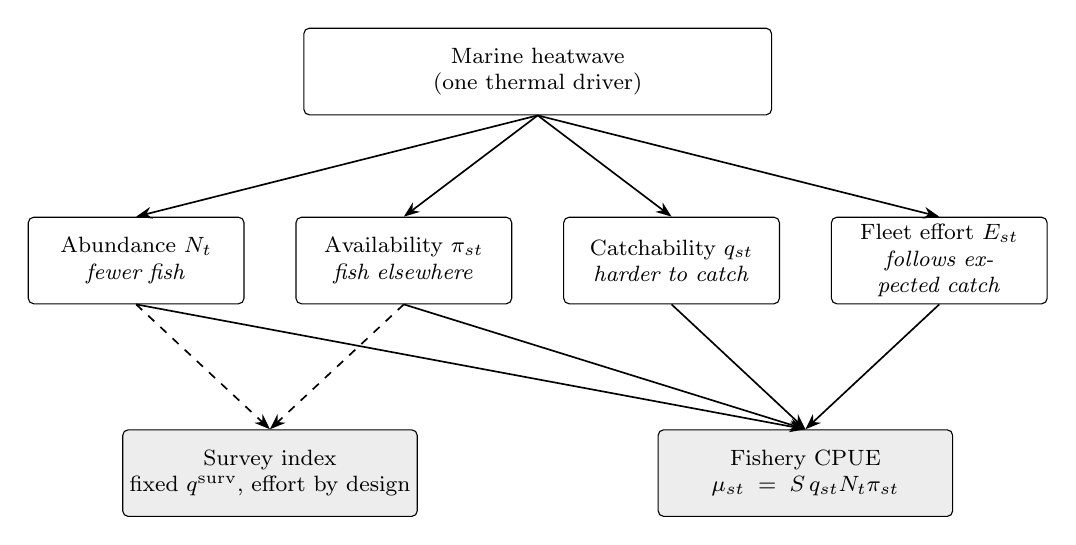
\begin{tikzpicture}[
  box/.style={draw, rounded corners=2pt, align=center, font=\footnotesize,
              text width=26mm, minimum height=11mm, inner sep=2pt},
  obs/.style={box, fill=black!7},
  arr/.style={-{Stealth[length=2mm]}, semithick}]
\node[box, text width=58mm] (mhw) at (51mm,24mm) {Marine heatwave\\(one thermal driver)};
\node[box] (N)  at (0mm,0mm)   {Abundance $N_t$\\\textit{fewer fish}};
\node[box] (pi) at (34mm,0mm)  {Availability $\pi_{st}$\\\textit{fish elsewhere}};
\node[box] (q)  at (68mm,0mm)  {Catchability $q_{st}$\\\textit{harder to catch}};
\node[box] (E)  at (102mm,0mm) {Fleet effort $E_{st}$\\\textit{follows expected catch}};
\node[obs, text width=36mm] (cpue) at (85mm,-27mm) {Fishery CPUE\\$\mu_{st}=S\,q_{st}N_t\pi_{st}$};
\node[obs, text width=36mm] (surv) at (17mm,-27mm) {Survey index\\fixed $q^{\text{surv}}$, effort by design};
\foreach \x in {N,pi,q,E} \draw[arr] (mhw.south) -- (\x.north);
\foreach \x in {N,pi,q,E} \draw[arr] (\x.south) -- (cpue.north);
\foreach \x in {N,pi} \draw[arr, dashed] (\x.south) -- (surv.north);
\end{tikzpicture}
\caption{Structure of the problem. One thermal driver acts on abundance, availability and catchability, and on where the fleet fishes. Fishery catch per unit effort depends on all of them through a product, so a change in total abundance and a change in catchability that is the same everywhere leave identical fishery data. The survey (dashed inputs) has fixed catchability and effort set by design, so it receives no input from catchability or the fleet; this is why it can separate abundance from catchability inside the sampling frame, and why it cannot see fish that leave the frame.}
\label{fig:schematic}
\end{figure}

Two clarifications shape what follows. The invariance concerns only the part of catchability that is the same everywhere. A change confined to part of the range, such as the warm edge, cannot be absorbed by a single monthly factor $a_t$, and it interacts with the spatial structure of the estimators in subtler ways, so we treat it as a separate mechanism. Structural non-identifiability, a flat direction in the likelihood that no amount of data can remove, is also distinct from practical non-identifiability, a likelihood that is curved but nearly flat at realistic sample sizes. Section~\ref{sec:res-ident} confirms the structural result numerically; the experiments that follow show how the practical problem behaves once the structural one is granted.

\subsection{The mechanisms as an experimental design}
\label{sec:design}

The operating model lets each heatwave response be switched on or off. Three are mechanisms through which a heatwave changes catch rate: abundance decline, redistribution (a change in availability) and uniform catchability loss. The fourth is a response of the fleet: during an event it contracts onto the grid cells it knows best, and the fished footprint shrinks. Together they form a full $2^4$ factorial of 16 scenarios. Treating the mechanisms as factors of a designed experiment, rather than as a handful of illustrative cases, lets us estimate the main effect of each mechanism on each estimator and the interactions among them, including those between fleet contraction and the biological mechanisms, which is where a sampling artefact would appear. We do not assume that the mechanisms combine additively; the interactions are estimated and reported. Four further scenarios add a catchability loss confined to the warm edge of the range, with and without redistribution and with and without fleet contraction, to test whether such a change can imitate real redistribution.

\subsection{What we estimate}
\label{sec:targets}

The quantity each index should recover is the effect of the heatwaves alone. To define it, every simulated data set is generated twice with the same random numbers: once with the heatwaves, and once with the heatwave anomaly removed while everything else (climatology, warming trend, noise, the fleet and its realised effort allocation) is held fixed. The difference between the two worlds is the heatwave effect, and we use two versions of it as targets,
\begin{equation}
\Delta_t = \log N_t - \log N^0_t, \qquad \Delta^{\vt{in}}_t = \Delta_t + \log\big(1-\pi^{\vt{out}}_t\big) - \log\big(1-\pi^{\vt{out},0}_t\big),
\label{eq:targets}
\end{equation}
where the superscript $0$ marks the world without heatwaves. The effect on total abundance, $\Delta_t$, answers the question ``how many fish did the heatwaves remove from the stock?''. The effect on in-frame abundance, $\Delta^{\vt{in}}_t$, adds the change in the log share of the stock inside the frame and answers ``how many fewer fish are there in the area we can sample?''. Each series is reduced to a single number, its slope on centred heatwave severity $I_t$ (Section~\ref{sec:om}) after allowing for a linear trend and a seasonal cycle,
\begin{equation}
y_t = \alpha + \beta\, I_t + \zeta_1 \tfrac{t}{T} + \zeta_2 \sin\tfrac{2\pi t}{12} + \zeta_3 \cos\tfrac{2\pi t}{12} + \xi_t ,
\label{eq:regression}
\end{equation}
with $y_t=\Delta_t$ giving the target $\beta$ and $y_t=\Delta^{\vt{in}}_t$ the target $\beta^{\vt{in}}$. Exactly the same regression is applied to every estimated log index, so that every estimate and every target refers to the same quantity.

The two targets differ only when a heatwave moves fish across the edge of the frame, and a survey of the frame can be unbiased only for the second. Which one a manager needs depends on whether the stock beyond the edge is still the stock being managed. Defining the targets by paired runs, rather than by the raw association of abundance with severity, is what separates the heatwave effect from background warming and seasonality. In our setting a simple regression of factual log abundance on severity gives almost the same value (within 0.002), so the distinction matters in principle but does not drive the results. Box~2 collects these and other key terms.

\begin{figure}[tb]
\centering
\fbox{\begin{minipage}{0.94\linewidth}
\small
\textbf{Box 2. Key terms}
\begin{description}\setlength{\itemsep}{1pt}
\item[Catch per unit effort (CPUE)] catch divided by the fishing effort that produced it, for example kilograms per trawl hour.
\item[Abundance] the number or biomass of fish in the whole stock.
\item[Availability] the share of the stock that is where the fleet fishes, and so could be caught.
\item[Catchability] the fraction of available fish taken by one unit of effort; it depends on gear, fish behaviour and how effort is deployed.
\item[Sampling frame] the area that the fishery and the survey can reach. Fish beyond its edge cannot be observed by either.
\item[In-frame abundance] abundance inside the sampling frame.
\item[Target (estimand)] the true quantity an index is meant to recover; here, the effect of the heatwaves alone on total or on in-frame abundance.
\item[Counterfactual] the same simulated world rerun without the heatwave anomaly. The difference between the two runs is the heatwave effect.
\item[Identifiable] two quantities are identifiable if different values of them produce different data. If they are not, no amount of data can separate them.
\item[Delta model] a two-part model of catch: one part for whether any fish are caught, one for how many when some are.
\item[Design-based survey index] an estimate that uses the known probabilities with which survey stations were chosen, rather than a model of where fish are.
\item[Centre of gravity] the density-weighted mean poleward position of the stock, or the catch-rate-weighted mean position of fishery catches.
\item[Scenario, replicate] a scenario is one combination of mechanisms; a replicate is one simulated data set from it. Results are averages over replicates.
\end{description}
\end{minipage}}
\end{figure}

% =============================================================================
\section{Methods}

\subsection{Overview of the simulation}

Each replicate simulates eight years (96 months) of a fishery on a $12\times12$ grid of 50~km cells, with an open poleward edge and a refuge band beyond it (Figure~\ref{fig:schematic}). Within each month the simulation runs in one sequence: the fleet allocates effort from its belief at the end of the previous month, abundance carries the removals implied by that effort, and catch is drawn from that abundance. The world without heatwaves (Section~\ref{sec:targets}) reruns the state process with the realised effort allocation and every random draw held fixed. Table~\ref{tab:settings} lists each symbol used below with its default value, and Table~\ref{tab:experiments} lists the experiments and the question each answers. Results are means over replicates. Scenarios share random numbers, so differences between scenarios are not inflated by simulation noise; the largest Monte Carlo standard error of any mean heatwave coefficient in the factorial is 0.0025.

\begin{table}[tbp]
\centering\footnotesize
\caption{Notation and default settings of the operating model, used in every experiment unless stated otherwise.}
\label{tab:settings}
\begin{tabular}{@{}l>{\raggedright\arraybackslash}p{8.4cm}>{\raggedright\arraybackslash}p{3.4cm}@{}}
\toprule
Component & Symbol and meaning & Value \\
\midrule
Domain & grid of $S = n_{\vt{lat}}\times n_{\vt{shelf}}$ cells; cell size & $12\times12$; 50~km \\
 & series length $T$ & 96 months \\
Temperature & mean climatology $\bar{T}$ & 18.0\,$^\circ$C \\
 & cooling with latitude $g_{\vt{lat}}$ and with cross-shelf position $g_{\vt{dep}}$ & 0.50 and 0.22\,$^\circ$C per band \\
 & seasonal amplitude $A$; phase $\varphi$ & 3.0\,$^\circ$C; 0.6 radians \\
 & warming trend $\omega$ & 0.05\,$^\circ$C per year \\
 & noise SD $\sigma_\varepsilon$; spatial kernel decay per cell $\rho_s$; temporal correlation $\rho_t$ & 0.40\,$^\circ$C; 0.55; 0.50 \\
Heatwaves & events per series $K$; duration & 6; 1 to 4 months \\
 & peak anomaly, mean (SD) & 2.2 (0.7)\,$^\circ$C \\
 & category one threshold $\tau$ & 1.0\,$^\circ$C \\
Thermal niche & optimum $T_{\vt{opt}}$; breadth $\sigma_{\vt{th}}$; stress threshold $T_{\vt{crit}}$ & 20.0; 1.9; 21.0\,$^\circ$C \\
Movement & adjustment rate $\rho_m$ & 0.55 per month \\
Abundance & recovery rate $r_0$; carrying capacity $K_{\vt{cap}}$; natural mortality $M$ & 0.09 per month; 1.0; 0 \\
 & sensitivity to thermal stress $\kappa$; response lag $L$ & 0.12; 0 months \\
 & fishing mortality scale $f$; process noise SD $\sigma_{\vt{proc}}$ & $1.2\times10^{-4}$; 0.020 \\
Catchability & base $q_0$; uniform loss $\delta_{\vt{dep}}$; warm-edge loss $\delta_{\vt{sp}}$; concentration $\gamma_{\vt{sp}}$ & 1.0; 0.07; 0.16; 1.40 \\
Fishery catch & encounter scale $a_0$; lognormal SD $\sigma_{\log}$ & 0.9; 0.6 \\
Fleet & total effort $E_{\vt{tot}}$; vessels; vessel efficiency SD & 60 units per month; 8; 0.25 \\
 & targeting strength $\beta_\mu$; contraction $\beta_J$; travel cost $\beta_{\vt{dist}}$ & 2.0; 0.8; 0.15 \\
 & learning rate $\psi$ (weight on the latest month's catch rate) & 0.5 \\
Survey & catchability $q^{\vt{surv}}$; encounter scale $a^{\vt{surv}}$; CV of positive tows & 1.0; 3.0; 0.45 \\
 & coverage $c$; frequency $k$; design & 0.10; monthly; simple random \\
\bottomrule
\end{tabular}
\end{table}

\begin{table}[tbp]
\centering\footnotesize
\caption{The experiments, the question each answers, and their size.}
\label{tab:experiments}
\begin{tabular}{@{}>{\raggedright\arraybackslash}p{0.16\linewidth}>{\raggedright\arraybackslash}p{0.35\linewidth}>{\raggedright\arraybackslash}p{0.32\linewidth}l@{}}
\toprule
Experiment & Question & Scenarios and replicates & Section \\
\midrule
Identifiability & Which heatwave responses can fishery data separate at all? & reduced likelihood on one simulated series & \ref{sec:res-ident} \\
Matched grid & Do different mixtures of decline and catchability loss give the same nominal coefficient? & $5\times5$ grid of decline rate $\kappa$ and catchability loss $\delta_{\vt{dep}}$ with fleet contraction, 80 replicates per point & \ref{sec:res-ident} \\
Factorial & Which index recovers which target under each combination of mechanisms? & 16 factorial and 4 warm-edge scenarios, 400 replicates each & \ref{sec:res-factorial}, \ref{sec:res-cog} \\
Survey design & How many stations, and how often, does a survey need? & 25 designs in the decline plus uniform catchability scenario with fleet contraction, 300 replicates each & \ref{sec:res-survey} \\
Frame geometry & Does the edge of the sampling frame change the answer? & 4 redistribution scenarios under 3 frame settings, 250 replicates each & \ref{sec:res-frame} \\
Temporal & Can a same-month model capture a lagged, cumulative decline? & one scenario with a 3-month lag, 300 replicates & \ref{sec:res-temporal} \\
Sensitivity & Which settings of the simulated world drive the results? & 15 parameters, 200 design points with 20 replicates each & \ref{sec:res-sens} \\
Diagnostic key & Can the joint pattern of the indices name the mechanism? & 5 factorial and 2 warm-edge scenarios with fleet contraction, split into training and test halves & \ref{sec:res-key} \\
\bottomrule
\end{tabular}
\end{table}

\subsection{Operating model}
\label{sec:om}

\subsubsection{Temperature and heatwaves}

Sea temperature in each grid cell and month is built from parts that can be removed one at a time, so that the world without heatwaves is well defined:
\begin{equation}
T_{st} = \underbrace{\bar{T} - g_{\vt{lat}}\,\ell_s - g_{\vt{dep}}\,c_s}_{\vt{climatology}} + \underbrace{A\sin\!\left(\tfrac{2\pi t}{12} - \varphi\right)}_{\vt{season}} + \underbrace{\omega\,\tfrac{t}{12}}_{\vt{trend}} + \underbrace{\varepsilon_{st}}_{\vt{noise}} + \underbrace{H_{st}}_{\vt{heatwave}} ,
\label{eq:temp}
\end{equation}
where $\ell_s$ and $c_s$ are the latitude band and cross-shelf band of cell $s$, so that the climatology cools poleward and offshore. The noise $\varepsilon_{st}$ has standard deviation $\sigma_\varepsilon$; it is smoothed in space by a kernel whose weight falls by a factor $\rho_s$ for each cell of distance, which makes neighbouring cells strongly correlated, and it is autocorrelated between consecutive months ($\rho_t$). The heatwave anomaly $H_{st}\ge0$ is zero outside events and is deleted in the world without heatwaves, whose temperature we write $T^0_{st}$.

Heatwaves follow a schedule of $K$ episodes per series, with random start months, durations of one to four months and peak anomalies near 2.2\,$^\circ$C; overlapping episodes merge. Within an episode the anomaly rises and decays smoothly. Its strength in each month is summarised by a severity index, the intensity above the category one threshold $\tau$ in units of that threshold,
\begin{equation}
J_t = \frac{\max(H_t - \tau,\ 0)}{\tau}, \qquad H_t = \frac{1}{S}\sum_s H_{st},
\label{eq:severity}
\end{equation}
which is zero in months without a heatwave and grows with its intensity. Catchability and the fleet respond to $\hat J_t$, the severity scaled to unit standard deviation over event months (and zero in a world without events); abundance and distribution respond to temperature itself, through the thermal niche. The estimators receive a different covariate, the centred and scaled severity $I_t = (J_t - \bar J)/\mathrm{sd}(J)$, so that no estimator is handed the sign of the true response through its covariate.

\subsubsection{Thermal suitability and movement}

Habitat suitability is a Gaussian function of the distance between local temperature and the thermal optimum,
\begin{equation}
h_{st} = \exp\!\left(-\frac{(T_{st}-T_{\vt{opt}})^2}{2\,\sigma_{\vt{th}}^2}\right),
\label{eq:suit}
\end{equation}
where $\sigma_{\vt{th}}$ sets the breadth of the niche. The sampling frame is open at its poleward edge. One latitude band beyond it lies a refuge whose temperature follows the same climatological gradient, season, trend and heatwave anomaly as the frame, $T^{\vt{ref}}_t = \bar T - g_{\vt{lat}}(n_{\vt{lat}}+1-\bar\ell) + A\sin(2\pi t/12-\varphi) + \omega t/12 + H_t$, with suitability $h^{\vt{ref}}_t$ from the same niche and the area of one band, $w^{\vt{ref}} = n_{\vt{shelf}}$. When redistribution is switched on, the stock moves part of the way each month toward the distribution that suitability alone would imply,
\begin{equation}
\pi_{st} = (1-\rho_m)\,\pi_{s,t-1} + \rho_m\,\tilde h_{st}, \qquad \pi^{\vt{out}}_t = (1-\rho_m)\,\pi^{\vt{out}}_{t-1} + \rho_m\,\tilde h^{\vt{ref}}_t,
\label{eq:move}
\end{equation}
with $\tilde h_{st} = h_{st}\big/\big(\sum_{s'}h_{s't} + w^{\vt{ref}}h^{\vt{ref}}_t\big)$, $\tilde h^{\vt{ref}}_t$ defined likewise, and the shares renormalised each month. The adjustment rate $\rho_m$ controls how quickly fish follow the suitability surface. Fish therefore leave the frame only when conditions beyond its edge are better than within it, which here happens in warm seasons and during events. When redistribution is switched off the shares stay at their climatological values. A refuge whose suitability is fixed in time is used as a comparison in Section~\ref{sec:res-frame}. Its suitability responds neither to the season nor to events, so it acts as a fixed reference: biomass leaves the frame toward it in normal conditions and returns when a heatwave warms the frame toward the thermal optimum.

\subsubsection{Abundance}

Abundance changes on the log scale through density-dependent recovery, natural and fishing mortality, and, when the decline mechanism is on, a response to the thermal stress the stock experienced $L$ months earlier:
\begin{equation}
\log N_t = \log N_{t-1} + r_0\!\left(1-\frac{N_{t-1}}{K_{\vt{cap}}}\right) - M - F_t - \kappa\,d_{t-L} + \eta_t, \qquad \eta_t\sim\mathcal{N}(0,\sigma^2_{\vt{proc}}),
\label{eq:abund}
\end{equation}
where $r_0$ is the intrinsic recovery rate, $K_{\vt{cap}}$ the carrying capacity, $M$ natural mortality and $\kappa$ the sensitivity of abundance to thermal stress. Fishing mortality is proportional to the expected catch per unit abundance implied by that month's effort,
\begin{equation}
F_t = f\,S\sum_{s=1}^{S} q_{st}\,\pi_{st}\,E_{st} \;\ge 0,
\label{eq:F}
\end{equation}
so it rises with the overlap between fleet and stock and falls when catchability falls. Thermal stress is weighted by where the stock is, so that only temperatures the fish actually experience count,
\begin{equation}
d_t = \sum_{s=1}^{S}\pi_{st}\,\max(T_{st}-T_{\vt{crit}},\ 0),
\label{eq:dose}
\end{equation}
with $T_{\vt{crit}}$ a stress threshold above the thermal optimum.

\subsubsection{Catchability}

Catchability has two parts: one that is the same everywhere, which is the part confounded with abundance, and one concentrated at the warm edge of the range,
\begin{equation}
q_{st} = q_0 \cdot \underbrace{\exp\!\left(-\delta_{\vt{dep}}\,\hat J_t\right)}_{\vt{uniform}} \cdot \underbrace{\exp\!\left(-\delta_{\vt{sp}}\,g_s\,\hat J_t\right)}_{\vt{warm edge}},
\label{eq:q}
\end{equation}
where $g_s = v_s/\bar v$ and $v_s = \max(1-\gamma_{\vt{sp}}\,y_s,\ 0)$, with $y_s$ the standardised poleward coordinate of the cell. The weight $g_s$ is largest at the warm, equatorward edge and averages one over the frame, so the second term concentrates the loss where water is warmest. Each part is switched on or off independently.

\subsection{How the fishery and the survey observe the stock}

\subsubsection{Fishery catch}

A grid cell that receives $E_{st}$ units of effort is fished with $E_{st}$ tows. It records at least one encounter with probability
\begin{equation}
p_{st} = 1-\exp(-a_0\,\mu_{st}\,E_{st}),
\label{eq:encounter}
\end{equation}
and, given an encounter, its catch rate (the mean over its tows) is lognormal with a variance that falls as effort rises,
\begin{equation}
Y_{st}\mid\vt{encounter} \sim \vt{Lognormal}\!\left(\log\frac{\mu_{st}}{p_{st}} - \frac{\sigma^2_{\log}}{2E_{st}},\ \frac{\sigma^2_{\log}}{E_{st}}\right), \qquad \Pr(Y_{st}=0) = 1-p_{st}.
\label{eq:catch}
\end{equation}
The two parts are matched so that the expected catch rate equals $\mu_{st}$ at any level of effort, $\mathbb{E}[Y_{st}] = p_{st}\cdot\mu_{st}/p_{st} = \mu_{st}$, and the zero catches that dominate real records enter every index that keeps them. Catch is drawn from the abundance of the same month after that month's removals, so observations and truth always refer to one state.

\subsubsection{Fleet behaviour}

Total monthly effort $E_{\vt{tot}}$ is shared among grid cells by a multinomial draw based on the fleet's belief at the end of the previous month and on the current month's heatwave severity,
\begin{equation}
(E_{1t},\dots,E_{St}) \sim \vt{Multinomial}\big(E_{\vt{tot}},\ w_{1t},\dots,w_{St}\big), \qquad w_{st} = \frac{\exp(u_{st})}{\sum_{s'}\exp(u_{s't})},
\label{eq:effort}
\end{equation}
where the attractiveness $u_{st}$ of a cell combines the fleet's belief about its catch rate, the cost of travel from port (with $\vt{dist}_s$ the scaled distance of the cell from port) and a vessel efficiency effect,
\begin{equation}
u_{st} = \beta_\mu\big(1+\beta_J\,\hat J_t\,\mathbf{1}\{\vt{contraction}\}\big)\,b_{s,t-1} - \beta_{\vt{dist}}\,\vt{dist}_s + \nu_{v(s)} .
\label{eq:score}
\end{equation}
Here $\beta_\mu$ is the strength of targeting and $\mathbf{1}\{\cdot\}$ equals one when fleet contraction is switched on. During an event the contraction term sharpens targeting, so effort concentrates on fewer, better-known cells and the fished footprint shrinks. Contraction has to enter as an interaction with targeting strength: a term added equally to every cell's score would cancel in the softmax of eq.~\eqref{eq:effort} and leave the allocation unchanged. The belief is a running blend of past and current experience,
\begin{equation}
b_{st} = (1-\psi)\,b_{s,t-1} + \psi\,z_{st},
\label{eq:belief}
\end{equation}
where $z_{st}$ is the log catch rate observed in cell $s$ in month $t$, standardised across cells, with the previous belief carried forward for cells left unfished, and $\psi$ is the weight placed on the latest month. Effort is generated rather than assumed, so catch rate is catch divided by effort throughout, as in a real fishery.

\subsubsection{Survey}

The fishery-independent survey visits $n=\max\{1,\operatorname{round}(cS)\}$ grid cells, drawn without replacement, once every $k$ months ($k=1$ monthly, 3 quarterly, 6 twice-yearly), either by simple random sampling or with equal allocation across latitude bands. Stratification places the same number of stations in each latitude band and needs at least one per band, so designs with fewer stations than bands revert to simple random sampling. Both designs give every cell the same inclusion probability, $p^{\vt{inc}} = n/S$, so stratification changes the variance of the estimator but not its form. Survey catches follow their own delta-lognormal model, with catchability $q^{\vt{surv}}$ and encounter scale $a^{\vt{surv}}$ fixed by protocol; neither responds to the heatwave. Its index is a Horvitz--Thompson estimate of the total, and its centre of gravity a Hájek ratio \citep{horvitz1952,sarndal1992},
\begin{equation}
\widehat B_t = \sum_{s\in\mathcal S_t}\frac{V_{st}}{p^{\vt{inc}}}, \qquad \widehat G_t = \frac{\sum_{s\in\mathcal S_t} y_s\,V_{st}}{\sum_{s\in\mathcal S_t}V_{st}},
\label{eq:survey}
\end{equation}
where $\mathcal S_t$ is the set of cells sampled in month $t$ and $V_{st}$ the survey catch. The total estimates $S\,q^{\vt{surv}}N_t(1-\pi^{\vt{out}}_t)$, the abundance inside the frame, not total abundance. In a month in which no station catches anything the total is zero and its logarithm undefined; such months are set to half the smallest positive total in the series, and their number is reported.

\subsection{Why a fishery-independent survey is not simply another catch rate}
\label{sec:why-survey}

A survey also records catch and effort, so it is fair to ask how a survey index differs from the CPUE whose failure this paper establishes. The arithmetic is the same: both divide catch by effort. What differs is how the effort is placed and whether catchability is fixed, and those two properties, not the ratio itself, decide whether an index tracks abundance.

\paragraph{Where effort goes.} Commercial effort follows the fish. In the model the allocation weights depend on last month's catch rates, on distance from port and, during events, on the contraction term, so the spatial distribution of effort is correlated with the very state being estimated. Survey stations are drawn with known, equal inclusion probabilities that do not depend on abundance. The commercial index averages over a footprint the fleet selects; the survey index is a probability-weighted average over a footprint fixed in advance, which is why it is computed as a Horvitz--Thompson total rather than as a raw ratio.

\paragraph{Whether catchability moves.} Commercial catchability responds to the heatwave, and its uniform component is exactly the quantity confounded with abundance in eq.~\eqref{eq:invariance}. By holding its gear, tow and protocol fixed, the survey keeps $q^{\vt{surv}}$ free of the severity-dependent factor, so its observations are not invariant under that change. A survey whose catchability drifted with the heatwave, or one standardised using the same fleet behaviour that creates the confounding, would recover no more than the fishery does.

\paragraph{Where it looks.} The fishery samples only where it fishes, and it stops fishing the warm edge precisely when catchability falls there. The survey samples the whole frame regardless of local catch rates, which is why its centre of gravity registers real redistribution but not a warm-edge catchability change.

\paragraph{What it cannot see.} A survey of the frame estimates in-frame abundance. If a heatwave moves fish across the frame edge, in-frame and total abundance diverge, and the survey, like the fishery, has no observation of the stock beyond it. This is why two targets are carried (Section~\ref{sec:targets}).

A survey index is privileged, then, not because it is a different kind of measurement, but because its effort is allocated independently of abundance and its catchability is held constant and known. These are design choices, and a survey that violated either would be as confounded as the fishery. Section~\ref{sec:res-survey} quantifies how much of a well-designed survey is needed; at very low coverage the survey fails through sampling variance, a different and more tractable failure than the structural confounding that defeats the fishery.

\subsection{Estimators and how they are compared}
\label{sec:estimators}

We compare a graded sequence of estimators, so that biases a better model can remove are separated from confounding that no model can remove. Each produces a monthly log index $y_t$.

\paragraph{Nominal index.} Total catch over total effort,
\begin{equation}
y^{\vt{nom}}_t = \log\frac{\sum_s Y_{st}E_{st}}{\sum_s E_{st}\,\mathbf{1}\{Y_{st}\ \vt{observed}\}},
\label{eq:nominal}
\end{equation}
the simplest index and the baseline for the others.

\paragraph{Positive-only index.} The mean log catch rate of positive catches after removing grid-cell and calendar-month means. It discards zero catches and stands in for a practice that delta models are meant to replace.

\paragraph{Delta index.} Two models with additive grid-cell and month effects, one for encounters and one for positive catches,
\begin{equation}
\operatorname{logit} p_{st} = a^{\vt{enc}}_s + m^{\vt{enc}}_t, \qquad \log Y_{st}\mid(Y_{st}>0) = \beta^{\vt{pos}}_0 + a^{\vt{pos}}_s + m^{\vt{pos}}_t + e_{st},
\label{eq:delta}
\end{equation}
with a light ridge penalty on the encounter effects of grid cells, since a cell in which fish are never encountered has no finite maximum-likelihood estimate. The index is the prediction over the complete grid at a fixed reference effort,
\begin{equation}
y^{\delta}_t = \log\left(\frac1S\sum_{s=1}^S \hat p_{st}\,\exp\!\big(\hat\beta^{\vt{pos}}_0 + \hat a^{\vt{pos}}_s + \hat m^{\vt{pos}}_t + \tfrac12\hat\sigma^2\big)\right),
\label{eq:deltaindex}
\end{equation}
so that it reflects modelled density rather than where effort happened to go. The fleet leaves most grid cells unfished in any month, and the prediction for those cells is an imputation; we report its share, together with a variant that averages only over the cells fished in each month.

\paragraph{Spatial delta index.} The delta index with a low-dimensional interaction between position and severity, $\mathbf{z}_s^{\top}\boldsymbol{\theta}\,I_t$ with $\mathbf{z}_s = (y_s, x_s)$ the poleward and offshore coordinates, added to each component. Its density surface can move with the event, which a purely additive model cannot do, so it also yields a centre of gravity \citep{thorson2016a}.

\paragraph{Survey index.} The design-based total of eq.~\eqref{eq:survey}.

Every index is reduced to a heatwave coefficient by the regression of eq.~\eqref{eq:regression}, the same regression that defines the targets. Standard errors use the Newey--West estimator with a Bartlett kernel and three lags \citep{newey1987}, which allows for autocorrelation in the monthly residuals and lets us report, for each estimator, the coverage of its 95 percent interval and its power to reject a zero effect. Accuracy is summarised by bias, root mean squared error (RMSE) and median absolute error against each target. A heatwave coefficient is the change in the log index for a one standard deviation increase in severity. At the sizes reported here it is close to a proportional change: a coefficient of $-0.023$ corresponds to a decline of about 2.3 percent per standard deviation of severity, and $-0.064$ to about 6 percent.

\subsection{Spatial and temporal diagnostics}
\label{sec:diagnostics}

\paragraph{Centre of gravity.} Three measures of where the stock is are compared with the true centre of gravity, $G_t = \sum_s y_s\,\pi_{st}\big/\sum_s\pi_{st}$. The fishery's centre of gravity weights the cells with positive catch by their catch rate,
\begin{equation}
G^{\vt{fish}}_t = \frac{\sum_{s\in\mathcal{P}_t} y_s\,Y_{st}}{\sum_{s\in\mathcal{P}_t} Y_{st}},
\label{eq:cog}
\end{equation}
where $\mathcal{P}_t$ is the set of fished cells with positive catch in month $t$. It describes where catch rates were high among the cells the fleet chose to fish; it indicates fishery use and is not an unbiased estimator of the stock's location. The centre of gravity of the spatial delta index surface estimates the stock's distribution, and the survey's is the Hájek ratio of eq.~\eqref{eq:survey}. Each is summarised by its event contrast, the mean poleward position during event months minus the mean outside them. Shifts are reported in kilometres: one unit of the standardised coordinate $y_s$ spans 3.46 latitude bands, or 173~km.

\paragraph{Lagged responses.} To ask whether a model without lags can capture a lagged, cumulative decline, the temporal experiment gives abundance a three-month lag ($L=3$), slower recovery ($r_0=0.05$), greater sensitivity ($\kappa=0.16$) and less process noise ($\sigma_{\vt{proc}}=0.010$), with decline and fleet contraction active and a monthly survey covering 20 percent of the grid. Two models are fitted to a centred target series $y_t$: a same-month model, $y_t = \alpha + \beta I_t + \xi_t$, and a distributed lag model in which severity in each of the previous $L_{\max}$ months has its own weight,
\begin{equation}
y_t = \alpha + \sum_{l=0}^{L_{\max}} w_l\,I_{t-l} + \xi_t, \qquad \vt{penalty } \lambda\sum_{l=2}^{L_{\max}}\left(w_l - 2w_{l-1} + w_{l-2}\right)^2,
\label{eq:dlag}
\end{equation}
with $L_{\max}=24$, long enough to cover the memory of the accumulating stock. The penalty favours smooth weight curves, and its strength $\lambda$ is chosen by generalised cross-validation \citep{craven1979},
\begin{equation}
\mathrm{GCV}(\lambda) = \frac{n\,\lVert \mathbf{y} - \mathbf{H}_\lambda \mathbf{y}\rVert^2}{\{n - \operatorname{tr}(\mathbf{H}_\lambda)\}^2},
\label{eq:gcv}
\end{equation}
where $\mathbf{H}_\lambda$ maps the observations to fitted values and its trace is the effective degrees of freedom. One target is the survey index with trend and season removed, which an analyst can observe; the other is the true heatwave effect, which bounds what any model of the lag structure could recover. The models are compared in sample and on blocked out-of-sample prediction over four contiguous blocks, with $\lambda$ re-selected inside each training block so that a held-out block never informs its own smoothing.

\paragraph{Global sensitivity.} Fifteen parameters are varied together over a Latin hypercube of 200 design points within the ranges of Table~\ref{tab:sensranges}, each point simulated with 20 replicates of the scenario in which all four mechanisms are active. For each outcome we report standardised regression coefficients, the slopes of a joint linear regression of the standardised outcome on the standardised parameters: the change in the outcome, in standard deviations, for a one standard deviation change in one parameter with the others held fixed.

\paragraph{A diagnostic key.} The mechanisms are expected to leave different joint signatures in four quantities: the heatwave coefficients of the delta and survey indices and the event contrasts of the fishery and survey centres of gravity. A coefficient is flagged when it is more negative, and a centre-of-gravity shift when it is more poleward, than the 95th percentile of that quantity's absolute value in no-effect training replicates. A decline flags both coefficients and neither centre of gravity; redistribution flags both centres of gravity but not the survey coefficient; uniform catchability loss flags the delta coefficient alone; warm-edge catchability loss flags the delta coefficient and the fishery centre of gravity; all four flags indicate a mixture, and any other pattern is returned as indeterminate. The key is learned and tested on seven scenarios with fleet contraction (no effect, decline, redistribution, uniform catchability loss, all three, warm-edge catchability loss, and warm-edge loss with redistribution, the last counted as redistribution), whose replicates are split at random into training and test halves.

\subsection{Computation}

All simulations, estimators, tables and figures are implemented in R 4.3.3. Replicate seeds are a deterministic function of the replicate index, so scenarios share random numbers and results are reproducible for a given R version. The code includes a test suite that checks, among other properties, that observations are drawn from the state the targets are defined on, that fishing mortality is never negative, that fleet contraction changes the effort allocation, and that the survey is unbiased for in-frame abundance.

% =============================================================================
\section{Results}

The operating model behaves as intended (Figure~\ref{fig:fields}). During a heatwave the domain warms, the stock contracts toward the cool poleward edge, and catchability falls at the warm edge, all emerging from the single thermal driver. The simulated data have the features that make real CPUE hard to interpret: a strongly seasonal temperature series punctuated by events, catch rates that are zero in 36 to 55 percent of fished cells (43 percent on average across scenarios) and right-skewed where positive, and a fished footprint that fluctuates with the fleet's beliefs (Figure~\ref{fig:S1}). Figure~\ref{fig:traj} makes the confounding concrete: under each mechanism the observed indices are plotted against both targets over time, and the nominal index departs from them event by event.

\begin{figure}[tbp]
\centering
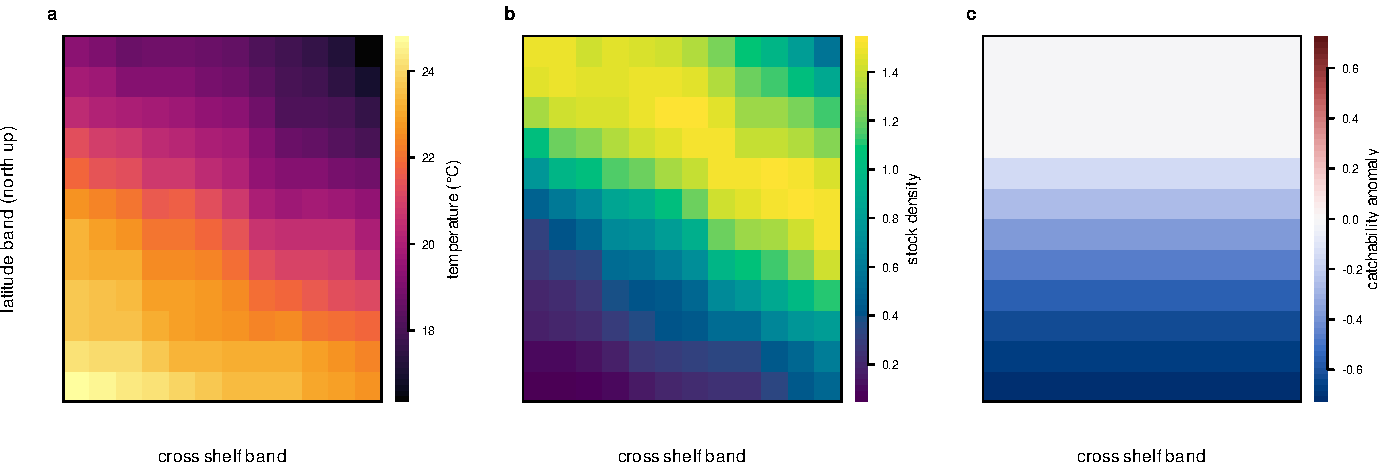
\includegraphics[width=\linewidth]{fig1_spatial_fields.pdf}
\caption{Spatial fields at the peak of a heatwave in a replicate with every mechanism active, including warm-edge catchability loss. (a) Sea temperature over the grid (north up, inshore at left). (b) Stock density, contracted toward the cool poleward edge. (c) Catchability relative to its pre-event level, reduced at the warm equatorward edge.}
\label{fig:fields}
\end{figure}

\begin{figure}[tbp]
\centering
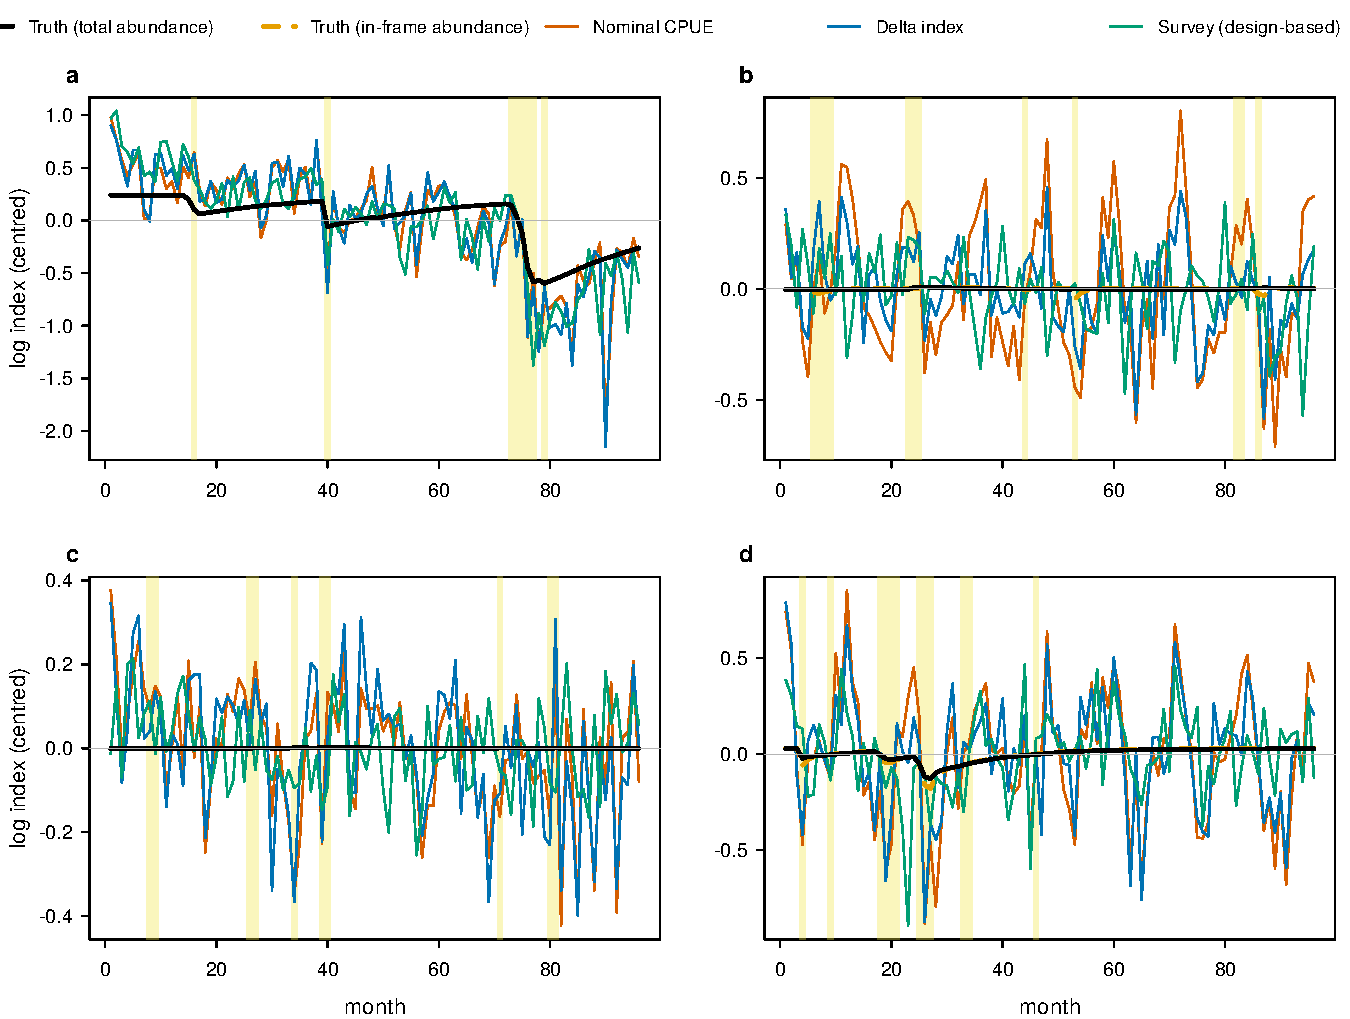
\includegraphics[width=\linewidth]{fig3_trajectories.pdf}
\caption{Index trajectories in one representative replicate of four scenarios, all with fleet contraction active: (a) abundance decline, (b) redistribution, (c) uniform catchability loss, (d) all three. Heatwave months are shaded. The heatwave effect on total abundance (black) and on in-frame abundance (grey dashed) are shown with the nominal, delta and survey indices, all centred. Under redistribution the two targets separate and the survey follows the in-frame target. Colours identify estimators consistently across all figures.}
\label{fig:traj}
\end{figure}

\subsection{Fishery data cannot split abundance from uniform catchability}
\label{sec:res-ident}

Fishery data carry no information about how a heatwave's effect is divided between abundance and uniform catchability (Figure~\ref{fig:ident}a). In a reduced likelihood with one slope for each, the fishery-only information matrix has eigenvalues of about 1209 and 0, the second zero to numerical precision, and the profile likelihood for the abundance slope varies by less than $2\times10^{-7}$ log-likelihood units over a range of 0.9 in the slope: it is flat. Adding survey observations with fixed catchability gives eigenvalues of about 2287 and 387 and a profile that falls by 322 log-likelihood units over the same range. These numbers follow from the form of the observation model rather than testing it independently; their value is in making the flat direction concrete.

A catchability change confined to the warm edge behaves differently. Adding a warm-edge catchability slope, which multiplies a weight that varies across grid cells, gives a three-parameter fishery information matrix with eigenvalues of about 2900, 186 and $5\times10^{-13}$. The only flat direction is the uniform one, and the profile for the warm-edge slope is curved from fishery data alone (Figure~\ref{fig:ident}b). With the survey added, all three eigenvalues are positive (3331, 1109 and 107).

The same flat direction appears in the full simulation. Across a grid of decline rates and uniform catchability losses, the nominal coefficient overstates the true effect everywhere except where both are zero, and the overstatement grows with catchability loss (Figure~\ref{fig:ident}c). Different mixtures produce nearly the same observation (Figure~\ref{fig:ident}d). Catchability loss without decline ($\kappa=0$, $\delta_{\vt{dep}}=0.07$; true effect $0.000$), a mixture of the two ($\kappa=0.06$, $\delta_{\vt{dep}}=0.035$; $-0.013$) and decline without catchability loss ($\kappa=0.12$, $\delta_{\vt{dep}}=0$; $-0.023$) give nominal coefficients of $-0.039$, $-0.036$ and $-0.030$. Survey coefficients separate them: $-0.002$, $-0.014$ and $-0.027$. Spatially structured catchability is identifiable without a survey; spatially uniform catchability is not. That distinction organises the rest of the results.

\begin{figure}[tbp]
\centering
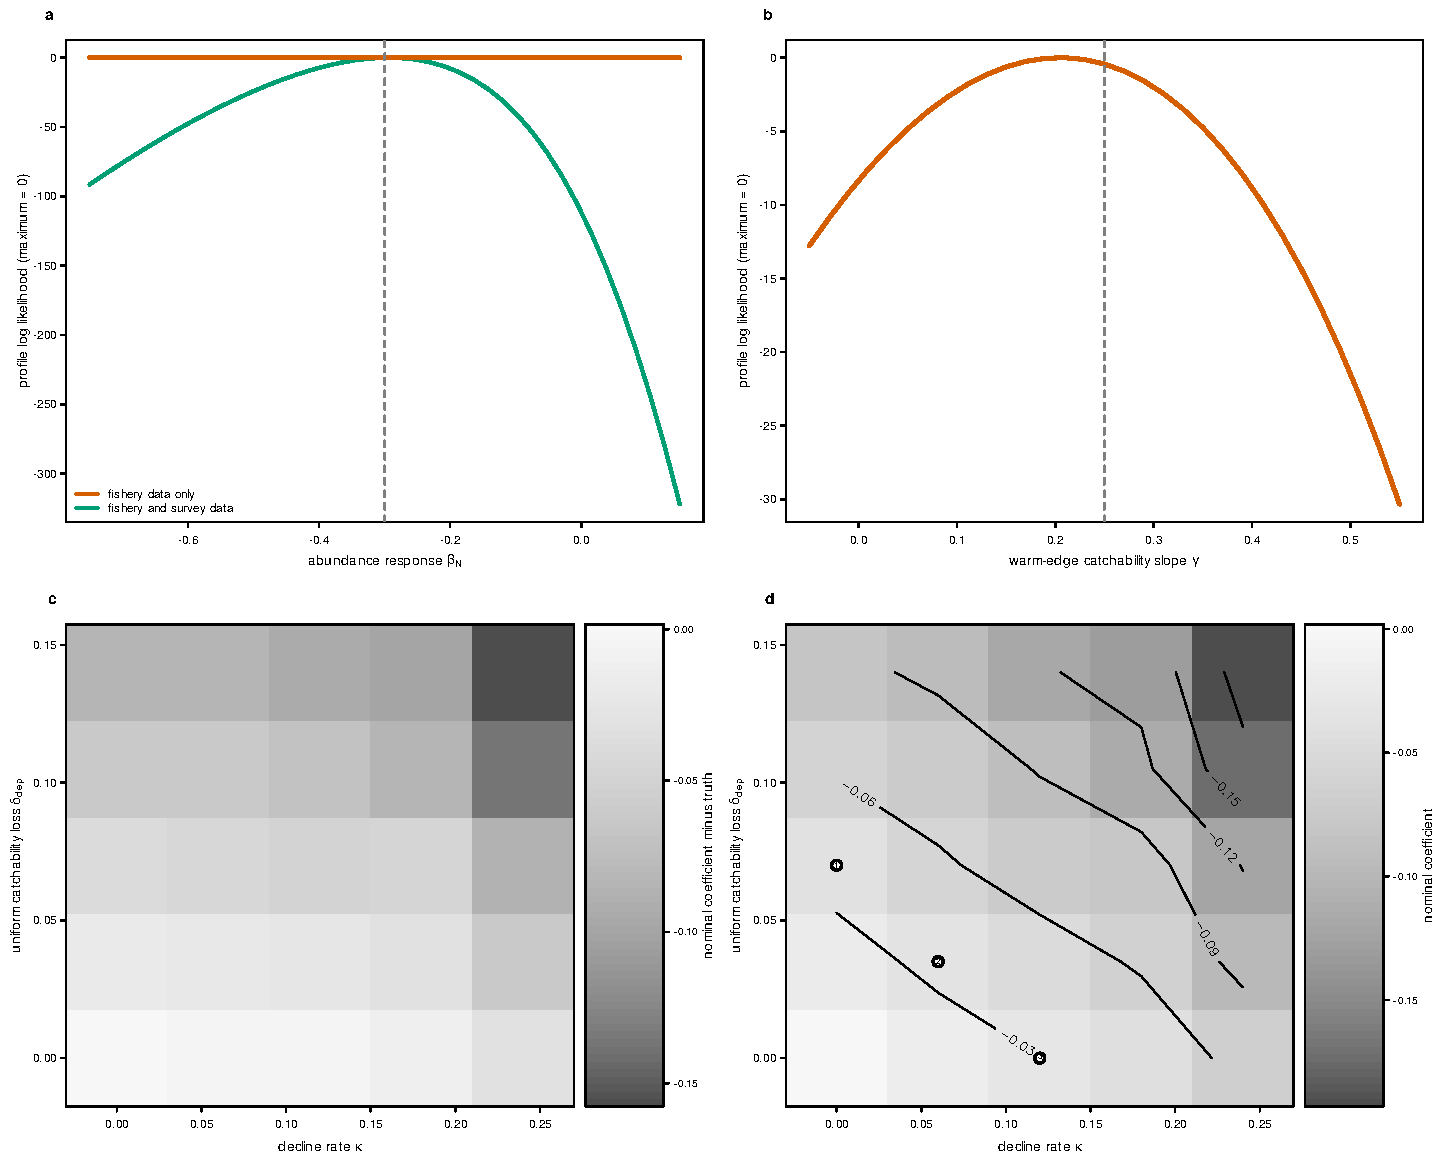
\includegraphics[width=\linewidth]{fig11_identifiability.pdf}
\caption{Fishery data cannot separate abundance from uniform catchability, but can detect a warm-edge catchability change. (a) Profile log likelihood of the abundance response $\beta_N$ from fishery data only (flat) and from fishery and survey data (curved); the dashed line marks the true value. (b) Profile log likelihood of the warm-edge catchability slope $\gamma$ from fishery data only, which is curved. (c) The nominal coefficient minus the true effect across a grid of decline rate $\kappa$ and uniform catchability loss $\delta_{\vt{dep}}$, with fleet contraction active (80 replicates per grid point). (d) The nominal coefficient over the same grid. Contours join combinations that give the same observed coefficient; the numbered points mark the three worlds compared in the text (1, catchability loss only; 2, both; 3, decline only).}
\label{fig:ident}
\end{figure}

\subsection{Which indices recover which target}
\label{sec:res-factorial}

Figure~\ref{fig:effects} and Table~\ref{tab:coef} report every estimator's heatwave coefficient in the scenarios with fleet contraction active, against both targets; Table~\ref{tab:coeffull} gives all 20 scenarios and Figure~\ref{fig:S2} shows how the key quantities vary across replicates. The same three patterns appear in every scenario.

\paragraph{A decline on its own is easy to detect.} With a true effect of $-0.023$, a decline of about 2.3 percent per standard deviation of severity, the nominal index reads $-0.022$, the delta index $-0.024$ and the survey $-0.024$. The positive-only index, which discards zero catches, is erratic rather than merely attenuated: it reads $-0.007$ without fleet contraction and $-0.026$ with it, because the zeros it discards carry the contraction's signal. The difficulty is that a heatwave need not change abundance alone, and the next two patterns show what happens when it does not.

\paragraph{Uniform catchability loss defeats every fishery index.} When catchability falls everywhere and abundance does not change, the nominal index reads $-0.039$, the delta index $-0.042$ and the spatial delta index $-0.041$; each reports a decline of about 4 percent per standard deviation of severity that did not happen. Against these, the survey reads $0.000$. When decline and catchability loss coincide, the nominal coefficient ($-0.064$) is 2.8 times the true effect ($-0.023$), the delta index is no better ($-0.067$), and the survey reads $-0.026$. This is the structural result of Section~\ref{sec:res-ident} appearing in finite samples, and it holds whatever the other mechanisms are doing.

\paragraph{Redistribution separates the two targets.} Under redistribution with no change in abundance, the effect on total abundance is zero, while in-frame abundance falls by 0.010 because an event moves 3 percent of the stock beyond the poleward edge. The survey, which samples only the frame, reads $-0.008$: it is unbiased for in-frame abundance and biased for total abundance by the share that left. Across all ten scenarios with redistribution, the survey's error against in-frame abundance is at most 0.003, comparable to the largest Monte Carlo standard error (0.0025), while its error against total abundance lies between $-0.007$ and $-0.012$ in every one. The spatial delta index, whose density surface can move with the event, tracks in-frame abundance when decline and redistribution coincide ($-0.025$ against $-0.025$) and under pure redistribution reads $-0.004$ against $-0.010$; in both cases it is far closer than the fixed-shape delta index ($-0.047$ and $-0.035$). It offers no protection once catchability also changes: with redistribution and uniform catchability loss together it reads $-0.045$ against an in-frame effect of $-0.010$. Redistribution therefore has a partial fishery-only remedy, available only when catchability is unchanged, whereas uniform catchability loss has none. The nominal index has no remedy for either: it reads $-0.045$ under pure redistribution, more than four times the in-frame effect, and the delta index, whose spatial shape is fixed, reads $-0.035$.

\begin{figure}[tbp]
\centering
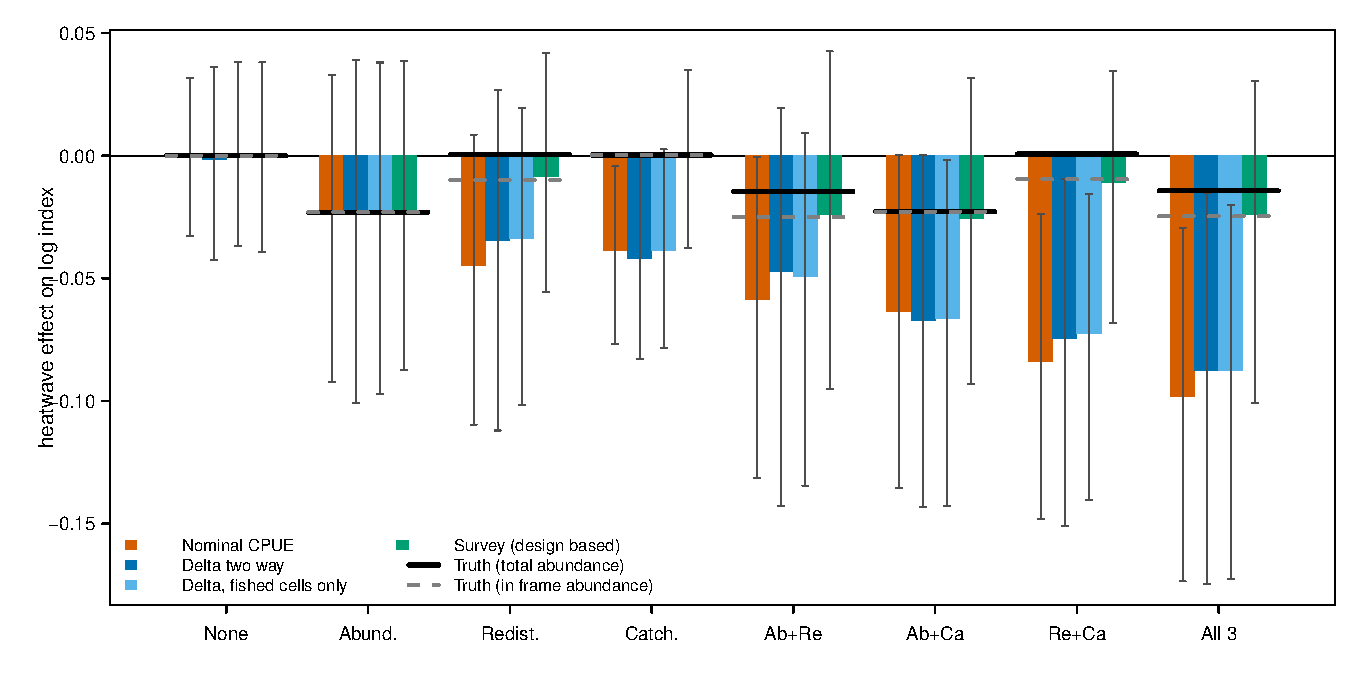
\includegraphics[width=\linewidth]{fig5_effect_by_case.pdf}
\caption{Heatwave coefficients for the eight combinations of abundance decline (Abund., Ab), redistribution (Redist., Re) and uniform catchability loss (Catch., Ca), all with fleet contraction active. Bars give the mean coefficient of each estimator over 400 replicates and whiskers the central 95 percent of replicates; the black line is the effect on total abundance and the grey dashed line the effect on in-frame abundance. The survey lands on the in-frame target in every scenario; no fishery index is robust to uniform catchability loss.}
\label{fig:effects}
\end{figure}

\begin{table}[tbp]
\centering\footnotesize
\setlength{\tabcolsep}{3.5pt}
\caption{Mean heatwave coefficient of each estimator by scenario, with fleet contraction active (400 replicates per scenario; largest Monte Carlo standard error 0.0025). The two target columns are the heatwave effects on total and on in-frame abundance; they differ only where redistribution moves fish across the frame edge. Table~\ref{tab:coeffull} adds the scenarios without fleet contraction.}
\label{tab:coef}
\begin{tabular}{@{}>{\raggedright\arraybackslash}p{3.2cm}rrrrrrrr@{}}
\toprule
 & \multicolumn{2}{c}{Target} & \multicolumn{6}{c}{Estimator} \\
\cmidrule(lr){2-3}\cmidrule(l){4-9}
 & & & & Positive- & & Delta, & Spatial & \\
Scenario & Total & In-frame & Nominal & only & Delta & fished & delta & Survey \\
\midrule
%%TAB:coef_main%%
\bottomrule
\end{tabular}
\end{table}

\paragraph{Fleet contraction on its own does little.} Without any biological mechanism, contraction is harmless (nominal coefficient 0.000 against a true effect of zero); it shrinks the fished footprint by 2.2 percent of the grid during events, and its interactions with the biological mechanisms are of order 0.003 (Table~\ref{tab:anova}). The fleet fishes only about 30 percent of grid cells in any month, so the full-grid delta index imputes about 70 percent of cells in calm and event months alike (70 and 72 percent with contraction active). The variant that averages only over fished cells differs from the full-grid index by at most 0.004 in any scenario, so imputation is not what drives the delta model's behaviour. The delta index fits converged in every replicate.

A linear model with all interactions, fitted to the replicate coefficients of the 16 factorial scenarios (Table~\ref{tab:anova}), shows how the mechanisms combine. Each main effect is the change produced by switching one mechanism on while the others are off, and each two-way term is the departure from additivity when two are on together. For the nominal index, redistribution alone shifts the coefficient by $-0.048$ and catchability loss alone by $-0.036$, more than abundance decline alone ($-0.024$); contraction alone shifts it by 0.002, and the largest two-way interaction, between decline and redistribution (0.009), is about a third of the smallest biological main effect. For the survey only decline ($-0.025$) and redistribution ($-0.010$) matter, and catchability loss has no effect ($-0.001$). The survey's decline-by-redistribution interaction (0.010) mirrors its target: when decline and redistribution coincide, the in-frame effect is $-0.025$ rather than the sum of the two separate effects. The mechanisms are close to additive on the coefficient scale, but not exactly, and reporting the interactions rather than assuming additivity is what licenses that statement.

\subsection{Only the survey separates movement from a warm-edge catchability artefact}
\label{sec:res-cog}

The centre of gravity separates real movement from a catchability artefact, but only when it is computed from the survey (Figure~\ref{fig:warmedge}, Table~\ref{tab:cog}). Under pure redistribution the stock's centre of gravity moves poleward by about 53~km during events. The fishery's centre of gravity moves by 45~km, the survey's by 49~km and that of the spatial delta index by 38~km, whereas the heatwave coefficient cannot register this movement at all, since the target on total abundance is zero. The warm-edge scenarios show why the fishery measure is not enough on its own. When catchability falls only at the warm edge, with no change in abundance or distribution, the fishery centre of gravity still moves poleward by 35~km, because catch rates fall in the warm-edge cells and the catch-rate-weighted mean moves away from them. The spatial delta surface shifts by about 32~km for the same reason, while the survey centre of gravity does not move (0.0~km). In the same scenario the nominal index reads $-0.102$ against a true effect of $0.001$, a spurious decline of about 10 percent per standard deviation of severity. Combined with real redistribution, the warm-edge loss exaggerates the fishery's shift (71~km against a true 53~km), while the survey stays close to the truth (49~km). Only the survey tells the two explanations apart.

\begin{figure}[tbp]
\centering
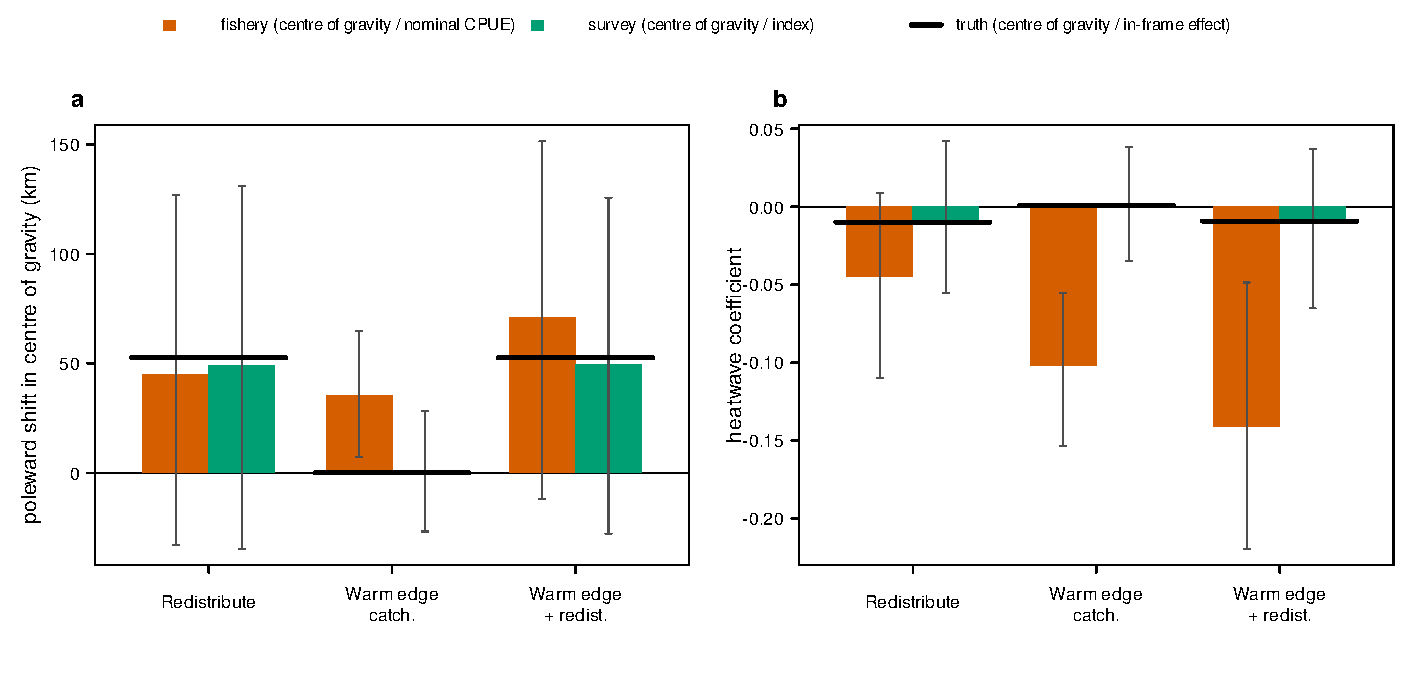
\includegraphics[width=\linewidth]{fig8_spatial_catchability.pdf}
\caption{Warm-edge catchability stress test, with fleet contraction active. (a) Poleward shift in the centre of gravity during events (km) for the fishery catch rates and for the survey, under redistribution, warm-edge catchability loss, and both; the black bar is the true shift. (b) Heatwave coefficient of the nominal index and the survey index for the same scenarios, against the effect on in-frame abundance (black). Whiskers show the central 95 percent of replicates. The survey centre of gravity moves only under real redistribution.}
\label{fig:warmedge}
\end{figure}

\begin{table}[tbp]
\centering\footnotesize
\caption{Centre-of-gravity diagnostics with fleet contraction active: event contrast of the poleward position (km) of the stock, the fishery catch rates, the spatial delta index surface and the survey, together with the event contrast of the share of the stock outside the frame (positive when fish leave) and of the fished footprint (share of grid cells fished).}
\label{tab:cog}
\begin{tabular}{@{}>{\raggedright\arraybackslash}p{3.6cm}rrrrrr@{}}
\toprule
 & \multicolumn{4}{c}{Centre of gravity shift} & \multicolumn{2}{c}{Change in} \\
\cmidrule(lr){2-5}\cmidrule(l){6-7}
Scenario & Stock & Fishery & Spatial delta & Survey & Share outside & Footprint \\
\midrule
%%TAB:centroids%%
\bottomrule
\end{tabular}
\end{table}

\subsection{What a survey must look like to recover the effect}
\label{sec:res-survey}

How large and how frequent must a survey be? We answer this in the scenario where the fishery is most misleading: a real decline combined with uniform catchability loss and fleet contraction (Figure~\ref{fig:design}, Table~\ref{tab:designcurve}). Without a survey, the nominal and delta indices have root mean squared errors of 0.054 and 0.061 against the true effect, and their 95 percent intervals contain the truth in only 53 and 51 percent of replicates: they are confidently wrong. A survey of 7 stations every month (84 tows a year) already has a lower error (0.042) than either fishery index; 14 stations a month bring the error to 0.028 with interval coverage of 89 percent, and further stations improve it only slowly. At 3 stations a month the survey is still competitive on median error but unreliable, because months in which no station catches anything are common (2.21 per series on average), and the log index for such a month carries no information.

Sampling frequency matters more than station count. A quarterly survey needs 29 stations per visit (116 tows a year) to bring its error (0.059) within the range of the fishery indices. Its error is dominated by occasional large misses, with root mean squared error two to five times the median absolute error at every station count, and its interval coverage falls to 79 percent, because 32 observations over eight years leave little room for the trend and seasonal terms. A twice-yearly survey samples the same two months every year, so it cannot separate the seasonal cycle from the event: the regression has to drop one seasonal term, the standard error becomes unreliable (coverage about 60 percent), and the apparent power of that design in Figure~\ref{fig:design}b is an artefact of undercoverage, which is why those points are drawn open. An annual survey, which we did not simulate, would provide eight observations of a single calendar month, too few to estimate an event-scale effect alongside a trend. Stratification by latitude band needs at least one station per band, so only the designs with 14 or more stations are stratified (smaller ones revert to simple random sampling); for those it changes the error by at most 0.001 (Table~\ref{tab:designcurve}), since the inclusion probabilities are the same and the variance between bands is small relative to the variance of a delta-lognormal catch within them. Doubling the survey CV to 0.90 raises the error of a 14-station monthly survey from 0.028 to 0.037, still below either fishery index.

Even a well-designed survey has limited power for an effect this small. At 14 stations a month the survey rejects a zero effect in 26 percent of replicates for a true decline of about 2.3 percent per standard deviation of severity, rising only to 34 percent at 58 stations, because the effect is small relative to the month-to-month variability of a catch rate. The nominal and delta indices reject a zero effect in 77 and 73 percent of replicates, but that is the power to detect a biased effect, not the true one. In this setting the survey is the only index that is right on average, and it is right with wide intervals.

\begin{figure}[tbp]
\centering
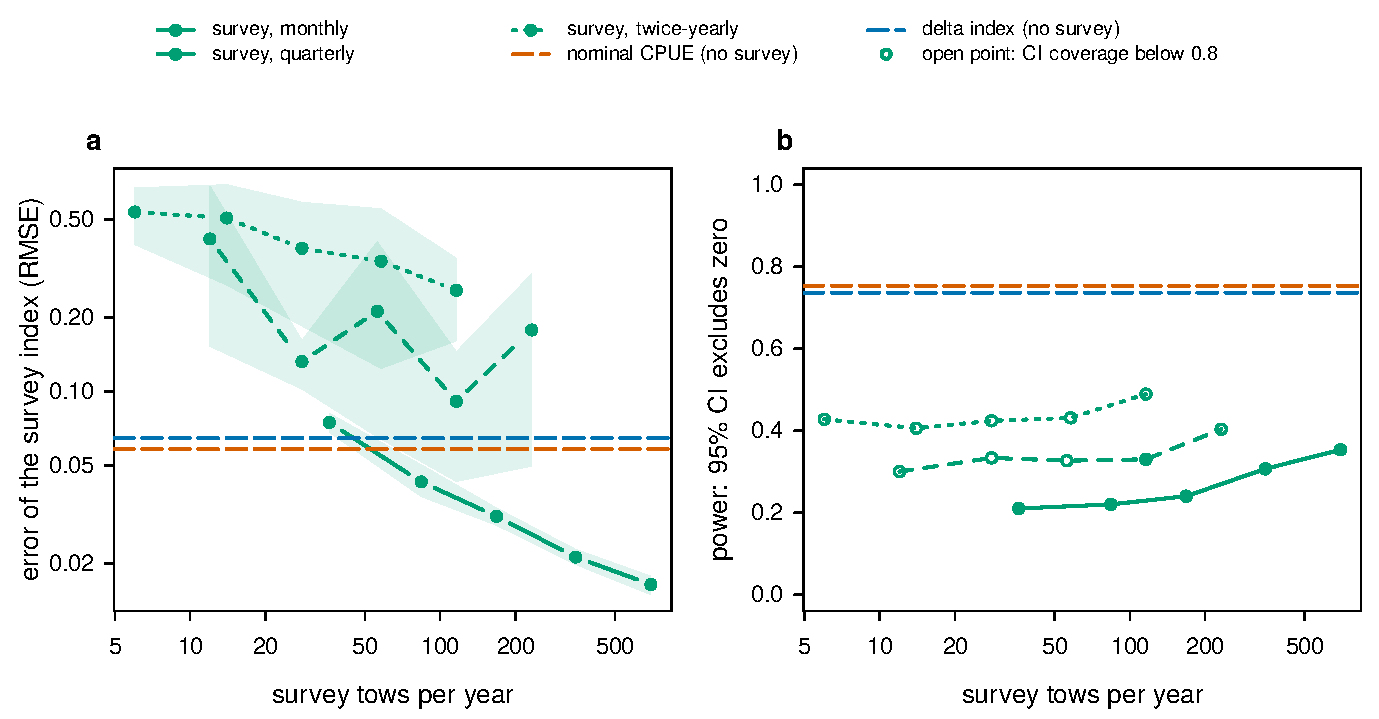
\includegraphics[width=\linewidth]{fig6_survey_coverage.pdf}
\caption{Survey design curve for the scenario with abundance decline, uniform catchability loss and fleet contraction (300 replicates per design). (a) Root mean squared error of the survey index against the true effect, by survey tows per year (both axes logarithmic), for monthly, quarterly and twice-yearly simple random surveys, with bootstrap 95 percent bands; the dashed horizontal lines are the two fishery indices, which do not use the survey. (b) Power to reject a zero effect. Open points mark designs whose 95 percent intervals contain the truth in fewer than 80 percent of replicates, for which power is not meaningful.}
\label{fig:design}
\end{figure}

\subsection{The edge of the frame sets the direction of the boundary flow}
\label{sec:res-frame}

Which way redistribution moves biomass across the frame edge depends on how the refuge beyond it is specified, and the survey follows that direction faithfully (Figure~\ref{fig:frame}, Table~\ref{tab:frame}; figures quoted with fleet contraction active). When the refuge experiences the same seasonal cycle, warming trend and heatwave anomaly as the frame, an event moves 3 percent of the stock beyond the poleward edge; the effect on in-frame abundance is $-0.010$ and the survey reads $-0.010$. When the refuge instead keeps a fixed, near-optimal suitability, the direction reverses. The heatwave warms the cool northern part of the frame toward the thermal optimum, the frame becomes more attractive than a refuge that never warms, and about 2.5 percent of the stock moves \emph{into} the frame during events; the in-frame effect is $0.007$ and the survey reads $0.008$. A refuge that does not warm acts as a thermostat, and the direction in which it moves biomass is a consequence of that specification rather than a property of heatwaves.

The nominal index, by contrast, falls under redistribution in every frame setting: $-0.036$ with a closed frame, $-0.045$ with a warming refuge and $-0.028$ with a static one. Its sign is therefore not set by the geometry of the frame. A plausible reason is that the fleet allocates effort from last month's catch rates, so its belief lags a moving stock and it keeps fishing where catch rates are falling. The sign of a redistribution artefact is thus not universal, a point we return to in the Discussion.

\begin{figure}[tbp]
\centering
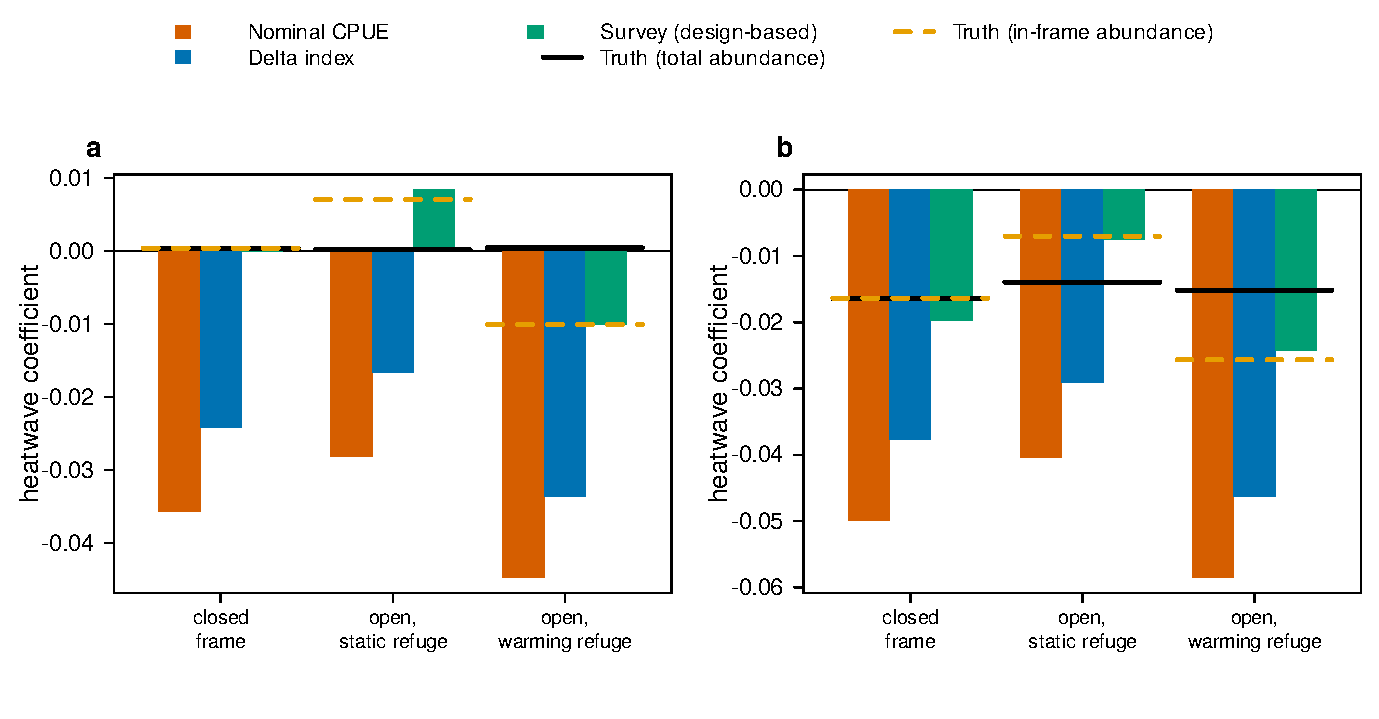
\includegraphics[width=\linewidth]{fig10_frame_geometry.pdf}
\caption{Frame geometry, with fleet contraction active (250 replicates per setting). (a) Redistribution only; (b) abundance decline and redistribution. Heatwave coefficients of the nominal, delta and survey indices against the effect on total abundance (black) and on in-frame abundance (grey dashed), for a closed frame, an open frame with a refuge of fixed suitability, and an open frame whose refuge warms with the frame (the default). The survey tracks in-frame abundance in every setting; which way in-frame abundance moves depends on whether the refuge warms.}
\label{fig:frame}
\end{figure}

\subsection{A distributed lag describes the lagged response but does not predict better}
\label{sec:res-temporal}

Can a model without lags capture a lagged, cumulative decline? Fitted to the detrended survey index, which is what an analyst can observe, the distributed lag raises the coefficient of determination from 0.02 to 0.18, using about 7 effective degrees of freedom, and its fitted series correlates with the true heatwave effect at 0.29, against 0.09 for the same-month model (Table~\ref{tab:temporal} reports correlations with the fitted target instead). The recovered lag weights spread their mass over the window, the delayed and cumulative shape of the true response (Figure~\ref{fig:temporal}). Fitted to the true effect itself, which shows the best that any such model could do, the distributed lag reaches a correlation of 0.55 against 0.15. A same-month model cannot represent a lagged, accumulating response, and the experiment confirms it.

Prediction is a different matter. On blocked out-of-sample prediction, with the smoothing parameter re-selected inside each training block, the distributed lag does not beat the same-month model on either target (root mean squared error 0.49 against 0.41 on the survey index), because its extra parameters add more variance than they remove bias. The distributed lag is the better description of the mechanism, not the better short-horizon predictor, and the two criteria should not be conflated.

\begin{figure}[tbp]
\centering
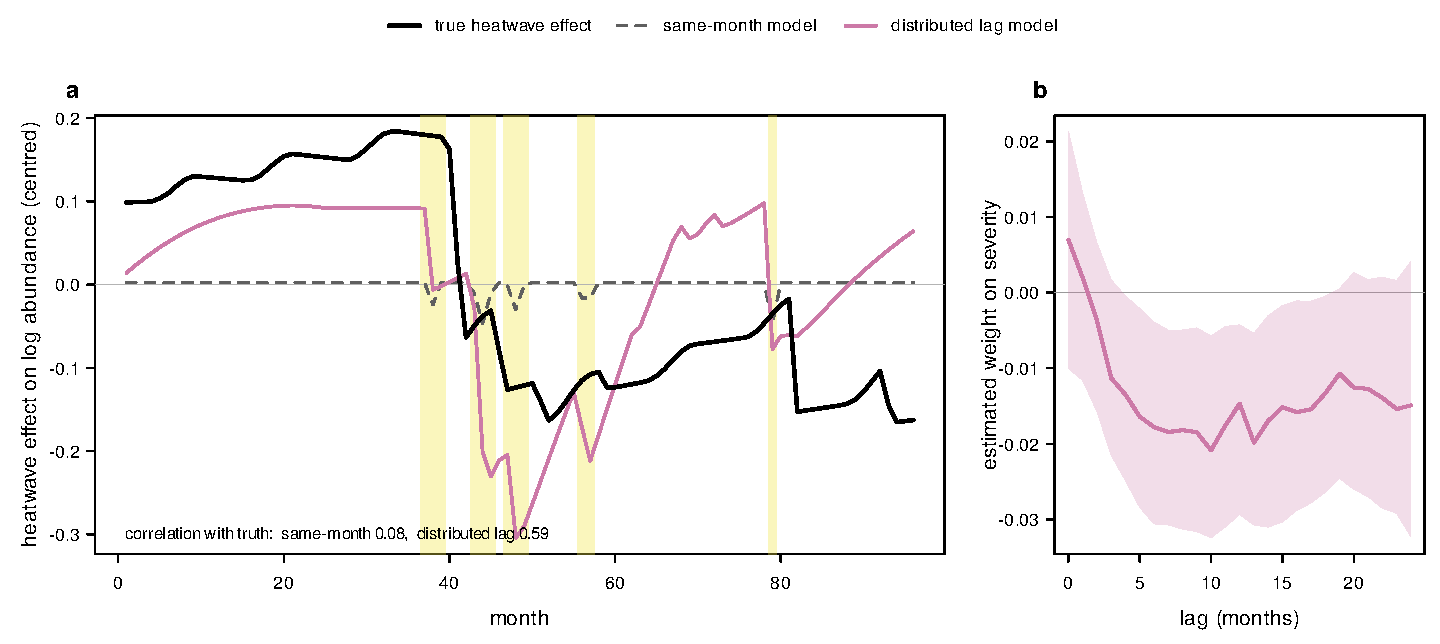
\includegraphics[width=\linewidth]{fig7_temporal.pdf}
\caption{Recovery of a lagged, cumulative decline from the observed survey index. (a) One replicate: the true heatwave effect on log abundance (black) and the fits of a same-month model (grey dashed) and a penalised distributed lag model (reddish purple) to the detrended survey index, on a common centred scale, with heatwave months shaded and the correlation of each fit with the truth annotated. (b) Estimated distributed lag weights across 300 replicates (mean and interquartile band), with smoothing chosen by generalised cross-validation.}
\label{fig:temporal}
\end{figure}

\begin{table}[tbp]
\centering\footnotesize
\caption{Temporal experiment (300 replicates): in-sample coefficient of determination ($R^2$), correlation of the fitted series with the target, blocked out-of-sample root mean squared error with smoothing re-selected in each training block, and effective degrees of freedom of the distributed lag, for two targets.}
\label{tab:temporal}
\begin{tabular}{@{}lrrrrrrr@{}}
\toprule
 & \multicolumn{2}{c}{$R^2$} & \multicolumn{2}{c}{Correlation} & \multicolumn{2}{c}{Out-of-sample RMSE} & \\
\cmidrule(lr){2-3}\cmidrule(lr){4-5}\cmidrule(lr){6-7}
Target & Same-month & Lag & Same-month & Lag & Same-month & Lag & Effective df \\
\midrule
%%TAB:temporal%%
\bottomrule
\end{tabular}
\end{table}

\subsection{What drives the results}
\label{sec:res-sens}

Which settings of the simulated world matter most (Figure~\ref{fig:sens}, Table~\ref{tab:sens})? The bias of the nominal index is governed above all by the size of the uniform catchability loss (standardised regression coefficient $-0.58$), the structural confound of Section~\ref{sec:res-ident}, and by the number of events ($-0.31$). Abundance sensitivity ($-0.20$), niche breadth ($0.16$) and the stock's movement rate ($-0.12$) follow; together the fifteen parameters explain 53 percent of the variation in the bias across the design. The strength of the fleet's contraction has almost no effect within the range tested ($0.004$), and the fleet's learning rate little ($0.07$). The survey's error against in-frame abundance depends on its own design, through coverage ($-0.44$) and encounter scale ($-0.36$), and on the size of the effect being estimated (abundance sensitivity, $0.33$). Its bias against total abundance depends on the settings that govern how much of the stock crosses the frame edge, chiefly the movement rate ($-0.38$), the number of events ($-0.36$), the warming trend ($-0.24$) and niche breadth ($0.18$); no fleet parameter has a coefficient larger than 0.09 in magnitude. A linear summary leaves much of the variation unexplained (47 percent for the nominal bias), so these coefficients rank the influences rather than predict outcomes at a given setting.

\begin{figure}[tbp]
\centering
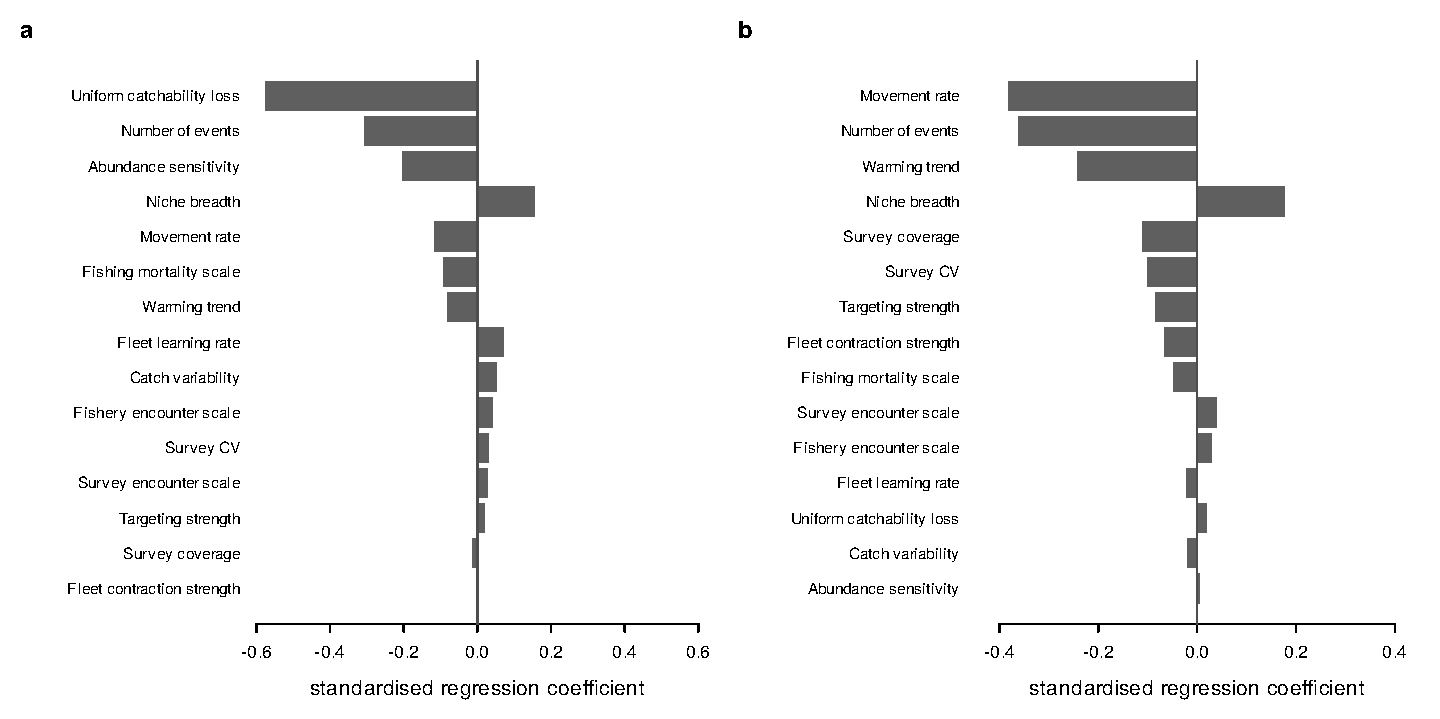
\includegraphics[width=\linewidth]{fig12_sensitivity.pdf}
\caption{Global sensitivity analysis. Standardised regression coefficients of (a) the bias of the nominal index against total abundance and (b) the bias of the survey index against total abundance, on the fifteen parameters of the design (200 design points, 20 replicates each, all mechanisms active). The parameters jointly explain 53 percent of the variation in (a) and 40 percent in (b).}
\label{fig:sens}
\end{figure}

\subsection{A diagnostic key and its error rate}
\label{sec:res-key}

The mechanisms leave different joint signatures across the indices, and a simple decision key built on them names the correct mechanism for 52 percent of test replicates across six classes, against about 17 percent expected by chance; it declines to classify 11 percent (Table~\ref{tab:key}). Warm-edge catchability loss is recognised in 83 percent of its test replicates and redistribution, a class that includes warm-edge loss combined with redistribution, in 56 percent. Abundance decline is the hardest class: only 25 of 194 replicates are classified correctly, and most are labelled as no effect (90) or indeterminate (51), because a decline of this size is often too small for the survey to detect (Section~\ref{sec:res-survey}). Uniform catchability loss is recognised in 55 percent of replicates and labelled as no effect in most of the rest. The key is useful but probabilistic, and its weakest point is a modest decline, which it more often misses than mislabels.

\begin{table}[tbp]
\centering\footnotesize
\scriptsize\setlength{\tabcolsep}{3.5pt}
\caption{Confusion matrix of the diagnostic key on held-out test replicates, with thresholds learned on a disjoint training half. Rows are the true mechanism, columns the assigned class.}
\label{tab:key}
\begin{tabular}{@{}lrrrrrrrrr@{}}
\toprule
& No & & Redistri- & Uniform & Warm-edge & & Indeter- & & Correct \\
Truth & effect & Decline & bution & catchability & catchability & Mixed & minate & Total & (\%) \\
\midrule
%%TAB:classifier%%
\bottomrule
\end{tabular}
\end{table}

% =============================================================================
\section{Discussion}

The central result is a negative one made precise and then made useful. Nominal and even well-standardised CPUE indices cannot, as a matter of the likelihood, separate a heatwave's effect on abundance from its effect on uniform catchability, because the two occupy a flat direction of the fishery likelihood. This is not a bias to be bounded; it is an identification failure that follows from the form of the observation model, and the finite-sample experiments show it operating in every scenario of the design. The difficulty is more than theoretical. A recent analysis of 248 marine heatwaves across North American and European continental shelves found that their effects on demersal fish biomass were often indistinguishable from natural and sampling variability, and were not consistently associated with community reorganisation \citep{fredston2023}. That result came from fishery-independent trawl surveys, which sharpens the motivation for the present work: if a heatwave signal is hard to detect even in survey data collected under a fixed design, reading it from commercial catch rates, in which abundance is entangled with availability and catchability, is harder still. Our power results make the same point from the other side, since a survey that is unbiased for the abundance effect still rejects a zero effect in only a minority of replicates at station counts at which it already outperforms the fishery. Table~\ref{tab:synthesis} collects what each mechanism does to catch rates and what resolves it.

\begin{table}[tbp]
\centering\footnotesize
\caption{What catch rates can and cannot reveal about a heatwave, and what resolves each case, in our simulation setting.}
\label{tab:synthesis}
\begin{tabular}{@{}>{\raggedright\arraybackslash}p{0.2\linewidth}>{\raggedright\arraybackslash}p{0.3\linewidth}>{\raggedright\arraybackslash}p{0.32\linewidth}l@{}}
\toprule
Mechanism & What fishery CPUE shows & What resolves it & Section \\
\midrule
Abundance decline alone & recovered by indices that keep zero catches & nothing further & \ref{sec:res-factorial} \\
Uniform catchability loss & read as a decline by every fishery index & a survey with fixed protocol and design-based effort & \ref{sec:res-ident}, \ref{sec:res-factorial} \\
Redistribution within the frame & false or exaggerated decline in the nominal and delta indices & spatial delta index, partly and only if catchability is unchanged; survey index and centre of gravity & \ref{sec:res-factorial}, \ref{sec:res-cog} \\
Redistribution across the frame edge & invisible to any index confined to the frame & a survey frame that extends beyond the historical range & \ref{sec:res-factorial}, \ref{sec:res-frame} \\
Warm-edge catchability loss & fishery centre of gravity shifts, imitating redistribution & survey centre of gravity, which does not move & \ref{sec:res-cog} \\
Lagged, cumulative decline & shape missed by a same-month model & distributed lag, as a description rather than a predictor & \ref{sec:res-temporal} \\
Survey requirement & & monthly sampling; 7 to 14 stations a month outperformed every fishery index; twice-yearly sampling cannot separate event from season & \ref{sec:res-survey} \\
\bottomrule
\end{tabular}
\end{table}

The constructive half of the framework is a mapping from each confounding mechanism to its remedy. Availability change has a partial fishery-only remedy: when catchability is unchanged, a spatially explicit standardisation whose density surface can move with the event removes most of the redistribution bias, and the centre of gravity of that surface captures most of the movement (38 of 53~km), although, like the fishery's, it also shifts under a warm-edge catchability loss. Uniform catchability change has no fishery-only remedy at all, since no covariate of the fishing operation observes it, and this is precisely the direction a survey is needed to pin down. Spatially structured catchability sits between the two. It is identifiable from fishery data, but it imitates redistribution in the fishery's own centre of gravity, and only the centre of gravity of an independent survey tells the two apart. That availability itself responds in complex ways during heatwaves is now well documented: modelling of fourteen top predators across four Northeast Pacific heatwaves found responses ranging from near-total loss of habitat to a twofold increase, varying by species and by event \citep{welch2023}, so the sign and size of an availability-driven CPUE signal cannot be assumed in advance. The bias induced by non-random, preferential allocation of commercial effort is itself an active area of study. Simulation work shows that fishery-dependent sampling in proportion to biomass can, under favourable conditions, recover indices comparable to those from random sampling, but degrades once the spatial mismatch between effort and abundance becomes severe \citep{ducharme2022}, and the difficulty of projecting distributions from such data has motivated dedicated methods \citep{karp2023}. Our results are consistent with that literature and add the identifiability perspective.

The survey deserves a more careful statement than ``it recovers abundance''. It helps because its effort is allocated independently of abundance and its catchability is fixed and known (Section~\ref{sec:why-survey}), and what it recovers is in-frame abundance. Whether that is the right target depends on the management question. If the stock beyond the boundary is lost to the fishery and its management, in-frame abundance is the right target and the survey is unbiased for it; if the boundary is an artefact of jurisdiction and the stock is expected to return, total abundance is the target and the survey will overstate a decline by the share that left. Which of the two a survey estimates is therefore a design decision, and in the frame geometry experiment even the direction of the difference depended on whether the refuge beyond the edge warmed with the frame (Section~\ref{sec:res-frame}). The practical recommendation is to decide which target a survey is meant to serve before it is designed, and to extend its frame beyond the historical range of the stock wherever total abundance is the question.

The confound matters further because the processes it entangles are correlated in nature rather than independent. Redistribution and abundance decline are widely treated as alternative readings of a falling local catch rate, one benign and one not, yet a global analysis of 2,572 marine fish population trends found that rapid poleward range shifts tend to coincide with local population declines rather than with stable abundance, so that a shifting stock is often also a declining one \citep{chaikin2024}. If redistribution and decline travel together, a CPUE change that appears to be ``just'' a distributional artefact may signal real loss, and the inability of a scalar index to tell them apart is not a conservative bias but a potentially dangerous one. This strengthens the case for the survey-based diagnostics developed here, which estimate the two processes separately rather than forcing an analyst to guess which one a catch rate reflects.

Redistribution lowered nominal CPUE in every frame setting, including a closed frame in which biomass merely concentrates, which is not what the hyperstability literature might lead one to expect \citep{harley2001,erisman2011}. Hyperstability requires a fleet that follows the stock into its contracted range, whereas the simulated fleet learns from last month's catch rates and so lags a stock that moves within a season. The sensitivity analysis is consistent with that explanation, although the effects are modest relative to catchability loss: the nominal bias grows with the stock's movement rate and shrinks slightly as the fleet learns faster, while the strength of its contraction during events has almost no effect. Hyperstability is a property of the fleet's response to the stock rather than of redistribution as such, and an attribution exercise should characterise that response rather than assume either sign. Integrated indices that combine fishery and survey data need similar care. By the argument of Section~\ref{sec:invariance}, a model that shares one month effect between the two streams would force that effect to absorb the fishery's catchability change, so it would recover only part of a decline unless the stream-specific effects were constrained, and fishery data cannot inform such a constraint. We did not fit such a model and instead benchmarked the survey and fishery indices separately.

For an agency, the results translate into decisions that must be taken before the next heatwave rather than after it. A survey has to be in place before the event, since a baseline cannot be collected afterwards. In our setting it needed to sample monthly to separate the event from the seasonal cycle; seven to fourteen stations a month were then enough to outperform every fishery index, whereas a quarterly survey needed 29 stations per visit merely to come within the range of the fishery indices, and a twice-yearly survey failed outright. Its frame should extend beyond the stock's historical range wherever total abundance is the question, and its gear and protocol should stay fixed through the event so that its catchability does not move with the heatwave. Fishery data remain valuable alongside such a survey. A spatially explicit standardisation of logbook data removed most of the redistribution bias when catchability did not change, and the fishery's centre of gravity, read against the survey's, distinguishes a warm-edge catchability change from movement. Recording where and how the fleet fished, and not only how much it caught, is what makes those comparisons possible.

Several limitations bound these claims. The operating model is deliberately simple: its grid, single environmental driver and thermal niche are caricatures of a real fishery, chosen so that the truth is known rather than to reproduce a particular stock. The structural result is general, since it follows from the form of the observation model rather than from any parameter value, but the finite-sample magnitudes, including the station counts, survey frequencies and error rates of the diagnostic key, are properties of this setting and should be read as orders of magnitude rather than transferable constants. Catch does not deplete a grid cell locally, so hyperstability through the sequential depletion of aggregations cannot arise. The delta index estimates one effect per grid cell and per month from sparse data, a setting in which maximum-likelihood estimates can be biased \citep[the incidental parameters problem;][]{neyman1948}; we assessed its behaviour by simulation rather than theory. The Newey--West intervals undercover somewhat for monthly surveys and badly for twice-yearly ones, which we report rather than correct. Our survey is idealised, with known, equal inclusion probabilities and fixed catchability; real surveys have their own catchability and design complications, which would raise the coverage required. The mechanisms are also treated as separable switches, whereas in a real heatwave they share a driver and may be correlated in ways the factorial does not capture, as the co-occurrence of range shift and decline noted above illustrates. These are directions for extension rather than threats to the core argument, which rests on the structure of the problem rather than on the details of the simulated world.

The framework applies to any fishery in which a heatwave signal is read from catch rates, and the natural next step is to condition it on a specific stock. The 2010--11 Western Australian heatwave, driven by an anomalously strong Leeuwin Current during an extreme La Ni\~{n}a \citep{pearce2013,feng2013}, offers such a setting, and Spanish mackerel in particular could anchor an operating model with real spatial structure, real effort and a real survey, turning the qualitative guidance here into stock-specific monitoring recommendations. That heatwave was followed by major recruitment failures in several invertebrate fisheries; managers responded with effort reductions and spatial or temporal closures, and the assessment of that response called for early detection of abundance change, preferably through pre-recruit surveys \citep{caputi2016}. Later work examined what governed the recovery of those stocks \citep{caputi2019}. Independent information of that kind is what this framework identifies as necessary, and its application to Western Australian stocks is the subject of a companion study.

% =============================================================================
\section{Conclusion}

Catch per unit effort cannot, on its own, tell whether a marine heatwave made a stock decline, move or merely become harder to catch, and this follows from the structure of fishery data rather than from a shortcoming of any particular standardisation. The way out is not a better model of the catch rate but a different kind of observation. A fishery-independent survey with design-allocated effort and protocol-fixed catchability restores identifiability, is unbiased for the abundance inside its frame, and separates real movement from a warm-edge catchability change through its centre of gravity. A spatially explicit standardisation of the fishery data removes most of the redistribution bias when catchability is unchanged, but none of the bias from uniform catchability change, and no index confined to the frame can see the share of a stock that an event moves beyond it. How much survey is needed is a quantitative question whose answer depends on frequency more than on station count. For a management agency facing the next heatwave, the data infrastructure needed to attribute its effect must be in place before the event, and the survey's frame, its frequency and the target it serves are design decisions that this framework can inform.

% =============================================================================
\section*{Acknowledgements}
% AUTHORS: add funding and acknowledgements.

\noindent\textit{Use of generative AI.} The authors used Claude (Anthropic; Fable 5.1 and Opus 5.5 models) to help write and test the R simulation code, generate figures, check references against their sources, and draft and edit the text. All code was executed in R 4.3.3, every reported number was reproduced by the authors from the archived code, and every reference was checked against the original publication. The authors take full responsibility for the content.
% AUTHORS: confirm that the reproduction and reference checks described above have been completed before submission, and adjust the statement to the journal's current policy.

\section*{Conflict of interest}
% AUTHORS: confirm.
The authors declare no conflict of interest.

\section*{Data availability statement}
This study uses no empirical data. All results, tables and figures are generated by simulation from the R code described in the Methods. The code, the simulated outputs underlying every reported number, and the scripts that reproduce the tables, figures and this manuscript are openly available on GitHub (\url{https://github.com/EAfrifa-Yamoah/Simulation-Recovery-of-Heatwave-Effect-}) and are permanently archived on Zenodo (\url{https://doi.org/10.5281/zenodo.23293721}; \citealp{awuah2026}).
% AUTHORS: the DOI above (...721) and the DOI in the reference list (...722) differ. If one is the
% Zenodo concept DOI and the other the version DOI, keep both; otherwise make them match.

% =============================================================================
\begin{thebibliography}{99}
\setlength{\itemsep}{2pt}

\bibitem[Afrifa-Yamoah et~al.(2026)]{afrifa2026}
Afrifa-Yamoah, E., Awuah-Mensah, Y. K., Bradshaw, S. and Mueller, U. (2026). Climate change impacts on fish-related ecosystem services: synthesis, network analysis, and strategic pathways for coordinated adaptation. \textit{Reviews in Fish Biology and Fisheries}, 36, 51.

\bibitem[Awuah-Mensah and Afrifa-Yamoah(2026)]{awuah2026}
Awuah-Mensah, Y. K. and Afrifa-Yamoah, E. (2026). Code: Declined, displaced, or just harder to catch? A simulation framework for attributing marine heatwave impacts on fished populations from catch per unit effort (Version v1.0.0) [Computer software]. \textit{Zenodo}. \url{https://doi.org/10.5281/zenodo.23293722}

\bibitem[Babcock et~al.(2019)]{babcock2019}
Babcock, R. C., Bustamante, R. H., Fulton, E. A. et al. (2019). Severe continental-scale impacts of climate change are happening now: extreme climate events impact marine habitat forming communities along 45\% of Australia's coast. \textit{Frontiers in Marine Science}, 6, 411.

\bibitem[Caputi et~al.(2016)]{caputi2016}
Caputi, N., Kangas, M., Denham, A., Feng, M., Pearce, A., Hetzel, Y. and Chandrapavan, A. (2016). Management adaptation of invertebrate fisheries to an extreme marine heat wave event at a global warming hot spot. \textit{Ecology and Evolution}, 6(11), 3583--3593.

\bibitem[Caputi et~al.(2019)]{caputi2019}
Caputi, N., Kangas, M., Chandrapavan, A., Hart, A., Feng, M., Marin, M. and de Lestang, S. (2019). Factors affecting the recovery of invertebrate stocks from the 2011 Western Australian extreme marine heatwave. \textit{Frontiers in Marine Science}, 6, 484.

\bibitem[Chaikin et~al.(2024)]{chaikin2024}
Chaikin, S., Riva, F., Marshall, K. E., Lessard, J.-P. and Belmaker, J. (2024). Marine fishes experiencing high-velocity range shifts may not be climate change winners. \textit{Nature Ecology \& Evolution}, 8(5), 936--946.

\bibitem[Cheung and Fr\"olicher(2020)]{cheung2020}
Cheung, W. W. L. and Fr\"olicher, T. L. (2020). Marine heatwaves exacerbate climate change impacts for fisheries in the northeast Pacific. \textit{Scientific Reports}, 10, 6678.

\bibitem[Craven and Wahba(1979)]{craven1979}
Craven, P. and Wahba, G. (1979). Smoothing noisy data with spline functions: estimating the correct degree of smoothing by the method of generalized cross-validation. \textit{Numerische Mathematik}, 31(4), 377--403.

\bibitem[Ducharme-Barth et~al.(2022)]{ducharme2022}
Ducharme-Barth, N. D., Gr\"uss, A., Vincent, M. T., Kiyofuji, H., Aoki, Y., Pilling, G., Hampton, J. and Thorson, J. T. (2022). Impacts of fisheries-dependent spatial sampling patterns on catch-per-unit-effort standardization: a simulation study and fishery application. \textit{Fisheries Research}, 246, 106169.

\bibitem[Erisman et~al.(2011)]{erisman2011}
Erisman, B. E., Allen, L. G., Claisse, J. T., Pondella, D. J., Miller, E. F. and Murray, J. H. (2011). The illusion of plenty: hyperstability masks collapses in two recreational fisheries that target fish spawning aggregations. \textit{Canadian Journal of Fisheries and Aquatic Sciences}, 68(10), 1705--1716.

\bibitem[Feng et~al.(2013)]{feng2013}
Feng, M., McPhaden, M. J., Xie, S.-P. and Hafner, J. (2013). La Ni\~{n}a forces unprecedented Leeuwin Current warming in 2011. \textit{Scientific Reports}, 3, 1277.

\bibitem[Fredston et~al.(2023)]{fredston2023}
Fredston, A. L., Cheung, W. W. L., Fr\"olicher, T. L. et al. (2023). Marine heatwaves are not a dominant driver of change in demersal fishes. \textit{Nature}, 621(7978), 324--329.

\bibitem[Fr\"olicher et~al.(2018)]{frolicher2018}
Fr\"olicher, T. L., Fischer, E. M. and Gruber, N. (2018). Marine heatwaves under global warming. \textit{Nature}, 560(7718), 360--364.

\bibitem[Fuster-Alonso et~al.(2024)]{fuster2024}
Fuster-Alonso, A., Conesa, D., Pennino, M. G. et al. (2024). Spatio-temporal sampling designs and dependence: implications for abundance indices. \textit{ICES Journal of Marine Science}, 81(5), 984--995.

\bibitem[Harley et~al.(2001)]{harley2001}
Harley, S. J., Myers, R. A. and Dunn, A. (2001). Is catch-per-unit-effort proportional to abundance? \textit{Canadian Journal of Fisheries and Aquatic Sciences}, 58(9), 1760--1772.

\bibitem[Hobday et~al.(2016)]{hobday2016}
Hobday, A. J., Alexander, L. V., Perkins, S. E. et al. (2016). A hierarchical approach to defining marine heatwaves. \textit{Progress in Oceanography}, 141, 227--238.

\bibitem[Horvitz and Thompson(1952)]{horvitz1952}
Horvitz, D. G. and Thompson, D. J. (1952). A generalization of sampling without replacement from a finite universe. \textit{Journal of the American Statistical Association}, 47(260), 663--685.

\bibitem[Hoyle et~al.(2024)]{hoyle2024}
Hoyle, S. D., Campbell, R. A., Ducharme-Barth, N. D. et al. (2024). Catch per unit effort modelling for stock assessment: a summary of good practices. \textit{Fisheries Research}, 269, 106860.

\bibitem[Karp et~al.(2023)]{karp2023}
Karp, M. A., Brodie, S., Smith, J. A. et al. (2023). Projecting species distributions using fishery-dependent data. \textit{Fish and Fisheries}, 24(1), 71--92.

\bibitem[Maunder and Punt(2004)]{maunder2004}
Maunder, M. N. and Punt, A. E. (2004). Standardizing catch and effort data: a review of recent approaches. \textit{Fisheries Research}, 70(2--3), 141--159.

\bibitem[Maunder et~al.(2006)]{maunder2006}
Maunder, M. N., Sibert, J. R., Fonteneau, A., Hampton, J., Kleiber, P. and Harley, S. J. (2006). Interpreting catch per unit effort data to assess the status of individual stocks and communities. \textit{ICES Journal of Marine Science}, 63(8), 1373--1385.

\bibitem[Maunder et~al.(2020)]{maunder2020}
Maunder, M. N., Thorson, J. T., Xu, H. et al. (2020). The need for spatio-temporal modeling to determine catch-per-unit effort based indices of abundance and associated composition data for inclusion in stock assessment models. \textit{Fisheries Research}, 229, 105594.

\bibitem[Newey and West(1987)]{newey1987}
Newey, W. K. and West, K. D. (1987). A simple, positive semi-definite, heteroskedasticity and autocorrelation consistent covariance matrix. \textit{Econometrica}, 55(3), 703--708.

\bibitem[Neyman and Scott(1948)]{neyman1948}
Neyman, J. and Scott, E. L. (1948). Consistent estimates based on partially consistent observations. \textit{Econometrica}, 16(1), 1--32.

\bibitem[Oliver et~al.(2018)]{oliver2018}
Oliver, E. C. J., Donat, M. G., Burrows, M. T. et al. (2018). Longer and more frequent marine heatwaves over the past century. \textit{Nature Communications}, 9, 1324.

\bibitem[Pearce and Feng(2013)]{pearce2013}
Pearce, A. F. and Feng, M. (2013). The rise and fall of the ``marine heat wave'' off Western Australia during the summer of 2010/2011. \textit{Journal of Marine Systems}, 111--112, 139--156.

\bibitem[S\"arndal et~al.(1992)]{sarndal1992}
S\"arndal, C.-E., Swensson, B. and Wretman, J. (1992). \textit{Model Assisted Survey Sampling}. Springer.

\bibitem[Smale et~al.(2019)]{smale2019}
Smale, D. A., Wernberg, T., Oliver, E. C. J. et al. (2019). Marine heatwaves threaten global biodiversity and the provision of ecosystem services. \textit{Nature Climate Change}, 9(4), 306--312.

\bibitem[Thorson(2019)]{thorson2019}
Thorson, J. T. (2019). Guidance for decisions using the Vector Autoregressive Spatio-Temporal (VAST) package in stock, ecosystem, habitat and climate assessments. \textit{Fisheries Research}, 210, 143--161.

\bibitem[Thorson and Barnett(2017)]{thorson2017}
Thorson, J. T. and Barnett, L. A. K. (2017). Comparing estimates of abundance trends and distribution shifts using single- and multispecies models of fishes and biogenic habitat. \textit{ICES Journal of Marine Science}, 74(5), 1311--1321.

\bibitem[Thorson et~al.(2020)]{thorson2020}
Thorson, J. T., Maunder, M. N. and Punt, A. E. (2020). The development of spatio-temporal models of fishery catch-per-unit-effort data to derive indices of relative abundance. \textit{Fisheries Research}, 230, 105611.

\bibitem[Thorson et~al.(2016a)]{thorson2016a}
Thorson, J. T., Pinsky, M. L. and Ward, E. J. (2016a). Model-based inference for estimating shifts in species distribution, area occupied and centre of gravity. \textit{Methods in Ecology and Evolution}, 7(8), 990--1002.

\bibitem[Thorson et~al.(2016b)]{thorson2016b}
Thorson, J. T., Rindorf, A., Gao, J., Hanselman, D. H. and Winker, H. (2016b). Density-dependent changes in effective area occupied for sea-bottom-associated marine fishes. \textit{Proceedings of the Royal Society B: Biological Sciences}, 283(1840), 20161853.

\bibitem[Thorson et~al.(2015)]{thorson2015}
Thorson, J. T., Shelton, A. O., Ward, E. J. and Skaug, H. J. (2015). Geostatistical delta-generalized linear mixed models improve precision for estimated abundance indices for West Coast groundfishes. \textit{ICES Journal of Marine Science}, 72(5), 1297--1310.

\bibitem[Welch et~al.(2023)]{welch2023}
Welch, H., Savoca, M. S., Brodie, S. et al. (2023). Impacts of marine heatwaves on top predator distributions are variable but predictable. \textit{Nature Communications}, 14, 5188.

\bibitem[Wernberg et~al.(2016)]{wernberg2016}
Wernberg, T., Bennett, S., Babcock, R. C. et al. (2016). Climate-driven regime shift of a temperate marine ecosystem. \textit{Science}, 353(6295), 169--172.

\bibitem[Wernberg et~al.(2013)]{wernberg2013}
Wernberg, T., Smale, D. A., Tuya, F., Thomsen, M. S., Langlois, T. J., de Bettignies, T., Bennett, S. and Rousseaux, C. S. (2013). An extreme climatic event alters ecosystem structure in a global biodiversity hotspot. \textit{Nature Climate Change}, 3(1), 78--82.

\end{thebibliography}

% =============================================================================
\clearpage
\appendix
\section*{Supporting Information}
\setcounter{table}{0}\renewcommand{\thetable}{S\arabic{table}}
\setcounter{figure}{0}\renewcommand{\thefigure}{S\arabic{figure}}

\begin{table}[htbp]
\centering\footnotesize
\caption{Ranges sampled by the global sensitivity design (Latin hypercube, 200 points); every other setting is as in Table~\ref{tab:settings}.}
\label{tab:sensranges}
\begin{tabular}{@{}llrr@{}}
\toprule
Parameter & Symbol & Default & Range \\
\midrule
Targeting strength & $\beta_\mu$ & 2.0 & 0.5 to 3.5 \\
Fleet contraction strength & $\beta_J$ & 0.8 & 0 to 1.6 \\
Fishery encounter scale & $a_0$ & 0.9 & 0.4 to 1.8 \\
Catch variability & $\sigma_{\log}$ & 0.6 & 0.35 to 1.0 \\
Survey CV & & 0.45 & 0.2 to 0.9 \\
Survey coverage & $c$ & 0.10 & 0.05 to 0.35 \\
Survey encounter scale & $a^{\vt{surv}}$ & 3.0 & 1.0 to 5.0 \\
Fleet learning rate & $\psi$ & 0.5 & 0.1 to 0.9 \\
Movement rate & $\rho_m$ & 0.55 & 0.2 to 0.95 \\
Number of events & $K$ & 6 & 3 to 10 \\
Warming trend ($^\circ$C per year) & $\omega$ & 0.05 & 0 to 0.20 \\
Abundance sensitivity & $\kappa$ & 0.12 & 0.04 to 0.24 \\
Uniform catchability loss & $\delta_{\vt{dep}}$ & 0.07 & 0 to 0.16 \\
Niche breadth ($^\circ$C) & $\sigma_{\vt{th}}$ & 1.9 & 1.4 to 3.0 \\
Fishing mortality scale & $f$ & $1.2\times10^{-4}$ & 0 to $3\times10^{-4}$ \\
\bottomrule
\end{tabular}
\end{table}

\begin{table}[htbp]
\centering\scriptsize
\setlength{\tabcolsep}{2.5pt}
\caption{Mean heatwave coefficient of each estimator in all 20 scenarios, with and without fleet contraction (400 replicates per scenario; largest Monte Carlo standard error 0.0025).}
\label{tab:coeffull}
\begin{tabular}{@{}>{\raggedright\arraybackslash}p{2.9cm}lrrrrrrrr@{}}
\toprule
 & & \multicolumn{2}{c}{Target} & \multicolumn{6}{c}{Estimator} \\
\cmidrule(lr){3-4}\cmidrule(l){5-10}
 & Con- & & & & Positive- & & Delta, & Spatial & \\
Scenario & traction & Total & In-frame & Nominal & only & Delta & fished & delta & Survey \\
\midrule
%%TAB:coef_full%%
\bottomrule
\end{tabular}
\end{table}

\begin{table}[htbp]
\centering\footnotesize
\caption{Main effects (one mechanism switched on, the others off) and two-way interactions from a linear model with all interactions fitted to the replicate heatwave coefficients of the $2^4$ factorial, with standard errors in parentheses, for the nominal, delta and survey indices. Three- and four-way terms were fitted but are not shown.}
\label{tab:anova}
\begin{tabular}{@{}lrrr@{}}
\toprule
Term & Nominal & Delta & Survey \\
\midrule
%%TAB:anova%%
\bottomrule
\end{tabular}
\end{table}

\begin{table}[htbp]
\centering\scriptsize
\setlength{\tabcolsep}{2.5pt}
\caption{Survey design curve in the scenario with abundance decline, uniform catchability loss and fleet contraction (300 replicates per design): root mean squared error (RMSE) of the survey index against the true effect with bootstrap 95 percent interval, median absolute error (MAE), mean number of months per series with no survey catch, 95 percent interval coverage and power. For twice-yearly designs 276 of the 300 replicates gave an estimable coefficient. Stratified designs with fewer than 12 stations revert to simple random sampling. Without a survey, the nominal and delta indices have RMSE %%FISHRMSE%%.}
\label{tab:designcurve}
\begin{tabular}{@{}lllrrrlrrrr@{}}
\toprule
& & & & Tows & & & & Empty & & \\
CV & Design & Frequency & Stations & per year & RMSE & 95\% interval & MAE & months & Coverage & Power \\
\midrule
%%TAB:design_curve%%
\bottomrule
\end{tabular}
\end{table}

\begin{table}[htbp]
\centering\scriptsize
\setlength{\tabcolsep}{3.5pt}
\caption{Frame geometry experiment (250 replicates per setting): both targets, the event contrast of the share of the stock outside the frame (positive when fish leave), and three indices, for the redistribution scenarios under three frame settings.}
\label{tab:frame}
\begin{tabular}{@{}>{\raggedright\arraybackslash}p{2.9cm}ll rrrrrr@{}}
\toprule
 & & & \multicolumn{2}{c}{Target} & & \multicolumn{3}{c}{Estimator} \\
\cmidrule(lr){4-5}\cmidrule(l){7-9}
Scenario & Contraction & Frame & Total & In-frame & Share outside & Nominal & Delta & Survey \\
\midrule
%%TAB:frame%%
\bottomrule
\end{tabular}
\end{table}

\begin{table}[htbp]
\centering\footnotesize
\caption{Standardised regression coefficients of four outcomes on the fifteen parameters of the sensitivity design. Design-level $R^2$ is %%SENSR2%% for the four columns.}
\label{tab:sens}
\begin{tabular}{@{}lrrrr@{}}
\toprule
 & Nominal & Survey error, & Survey bias, & Nominal \\
Parameter & index bias & in-frame & total & wrong sign \\
\midrule
%%TAB:sensitivity%%
\bottomrule
\end{tabular}
\end{table}

\clearpage
\begin{figure}[htbp]
\centering
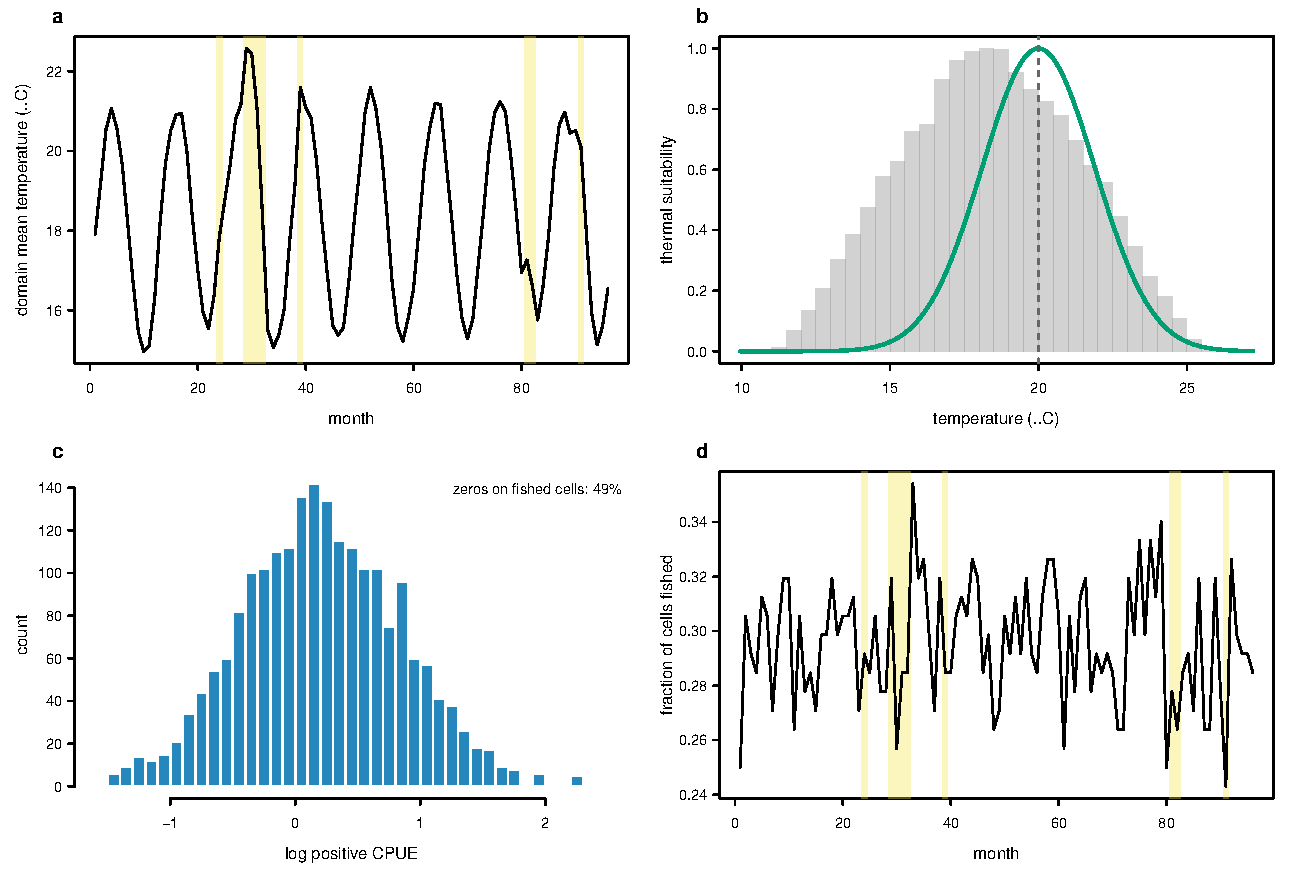
\includegraphics[width=0.9\linewidth]{fig2_data_distributions.pdf}
\caption{Simulated observations in a replicate with every mechanism active. (a) Mean temperature over the grid, with heatwave months shaded. (b) The thermal suitability curve, with the distribution of realised temperatures behind it. (c) Distribution of log positive CPUE, with the share of fished grid cells returning zero catch. (d) Share of grid cells fished in each month.}
\label{fig:S1}
\end{figure}

\begin{figure}[htbp]
\centering
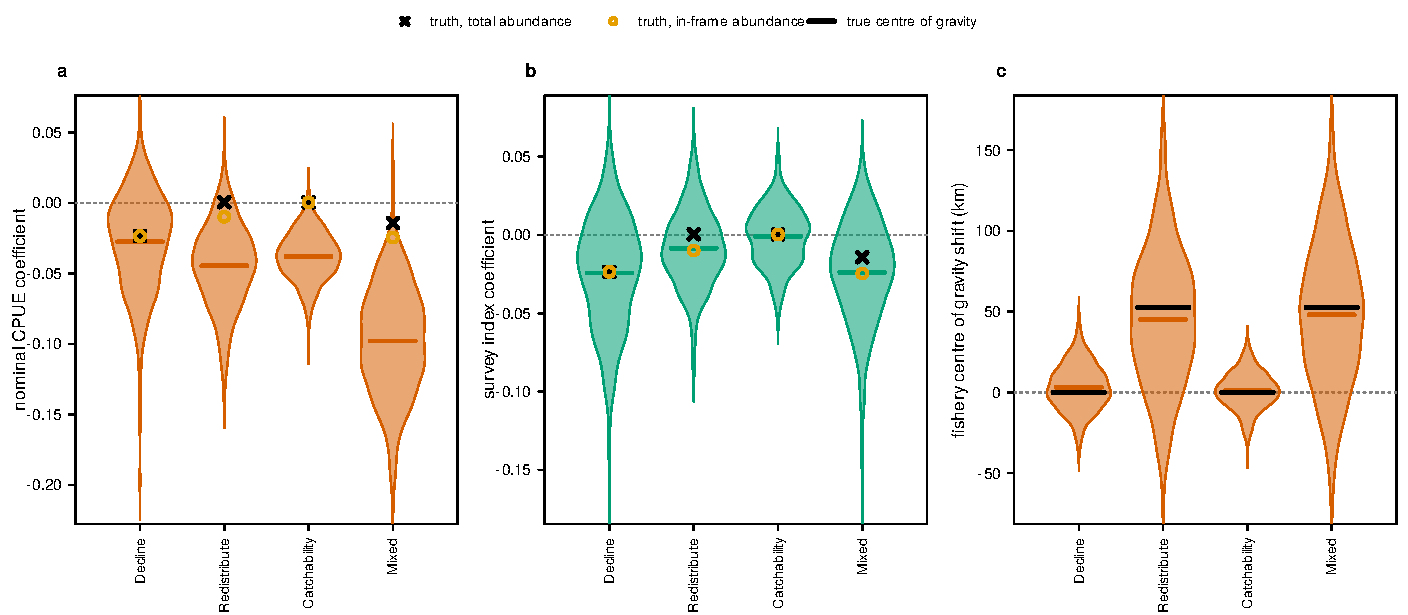
\includegraphics[width=\linewidth]{fig4_sampling_distributions.pdf}
\caption{Sampling distributions over 400 replicates for four scenarios with fleet contraction active (violins, with the replicate mean as a bar). (a) Nominal CPUE coefficient; (b) survey index coefficient; in both, the effect on total abundance is the black cross and the effect on in-frame abundance the grey circle. (c) Shift in the fishery's centre of gravity during events (km), with the true shift as the black bar.}
\label{fig:S2}
\end{figure}

\end{document}
